\chapter{Discrete Sampling and Intercalation of Periodic Signals}
\label{chap:sampling}
\markboth{Discrete sampling approximation, congruence angles and intercalation}{Discrete sampling approximation, congruence angles and intercalation}

\begin{remark}[Positioning and main line of this chapter]\label{rem:discrete_periodic_chapter_positioning}
This chapter is the \textbf{discrete implementation} of the `Periodic Functions and Groups with Periodic Orbits' chapter, but its main line is upgraded from `discrete periodic functions' to \textbf{discrete sampling approximation}, and further upgraded to \textbf{congruence-angle sampling approximation}. Its starting point is an engineering fact: any computable description of a continuous object must pass through the three steps of \textbf{sampling}, \textbf{truncation} and (when necessary) \textbf{intercalation}. Each of the three steps introduces a class of error---aliasing, spectral leakage, approximation error---and all three are governed by one and the same discrete structure, and are ultimately characterised uniformly by the congruence angle.

The core claims of this chapter are four:
\begin{enumerate}[label=(\roman*)]
    \item \textbf{An epicycle group is the rotational decomposition of a periodic signal}: a continuous Fourier series may be regarded as the superposition of a family of uniformly rotating epicycles; after discrete sampling, the epicycle group degenerates into finitely or countably many discrete rotational components.
    \item \textbf{Intercalation is not a trick of calendars, but an active commensuration device in discrete sampling approximation}; it presses the sole root of spectral leakage, namely `the number of periods inside the window being non-integral', down to the order $O(M^{-2})$ by means of the best continued-fraction approximation.
    \item \textbf{The congruence angle is the unified language of sampling, leakage, intercalation and the Chinese remainder theorem}; it upgrades `phase' from a continuous angle to an `equivalence class modulo a subperiod', so that single-period problems generalise naturally to multi-period joint problems.
    \item \textbf{Intercalation is the optimal compensation of congruence-angle error; the Chinese remainder theorem is the algebraic form of congruence-angle reconstruction; spectral leakage is the frequency-domain manifestation of congruence-angle non-closure.}
\end{enumerate}

\textbf{Parallel structure}:
\[
\begin{aligned}
\text{Continuous chapter} && \text{This chapter (discrete sampling approximation)} \\
\text{Periodic function } x(t) && \text{Sampling sequence } f(n)=x(n\Delta x) \\
\text{Group with periodic orbits } T_x\mathbb{Z} && \text{Group with periodic orbits } T_0\mathbb{Z}\subset\mathbb{Z} \\
\text{Fourier series } \sum_k c_k e^{i\omega_k t} && \text{Epicycle group } \mathcal{E}=\{(A_j,\omega_j,\phi_j)\} \\
\text{Discrete Fourier transform (DFT)} && \text{Finite epicycle group and DFT} \\
\text{Spectrum } |c_k| && \text{Window spectrum and Dirichlet kernel} \\
\text{Periodic convolution} && \text{Circular convolution, congruence-angle circular convolution and intercalation window}
\end{aligned}
\]

\textbf{The eight themes of this chapter}: translation---the sampling lattice $\Delta x\mathbb{Z}$ and translation invariance; scaling---the sampling rate $\nu_s$ and the fixed-length scale $T_0$; rotation---the discrete phase operator $\mathcal{O}_k^{(T)}=e^{i2\pi k/T}$, the epicycle group and the congruence angle; conservation---the discrete Parseval identity; symmetry---the even symmetry of the window spectrum and the spectral symmetry of a real sequence; closure---circular convolution, congruence-angle closure and the intercalation window; period---the duality between the number of periods in the window and the offset $\delta$, and the multi-period congruence-angle non-closure; algorithms---continued-fraction expansion, the balanced intercalation sequence and fast congruence-angle reconstruction.

\textbf{Reading route}: Section \ref{sec:sampling_basics} establishes the three elements of sampling; Section \ref{sec:epicycle_system} introduces the epicycle group; Section \ref{sec:window_dirichlet} gives the complete mechanism of leakage; Section \ref{sec:aliasing} discusses the price of the sampling rate; Section \ref{sec:bounded_approximation} establishes the upper and lower approximation and the optimality of continued fractions; Section \ref{sec:window_functions} gives the sidelobe control of window functions; Section \ref{sec:commensurability_intercalation} answers `why intercalation can suppress leakage'; Section \ref{sec:congruence_angle_crt} introduces the congruence angle and the generalised Chinese remainder theorem; Section \ref{sec:congruence_angle_intercalation} upgrades intercalation to multi-period joint suppression; Section \ref{sec:congruence_angle_algorithms} gives congruence-angle algorithms and complexity; Sections \ref{sec:intercalation_algorithms} to \ref{sec:ch17_interfaces} give the implementation, the calendar unification and the chapter interfaces.
\end{remark}

\begin{figure}[htbp]
\centering
\begin{tikzpicture}[>=Stealth, thick, scale=0.95]
% continuous signal
\draw[->] (-0.3,0) -- (9,0) node[right] {$t$};
\draw[->] (0,-1.4) -- (0,1.6) node[above] {$x(t)$};
\draw[blue, very thick, domain=0:8.6, samples=200] plot (\x, {0.9*sin(deg(1.6*\x))});
% sampling points
\foreach \n in {0,1,...,17} {
  \pgfmathsetmacro{\x}{\n*0.5}
  \pgfmathsetmacro{\y}{0.9*sin(1.6*\x r)}
  \fill[red] (\x,\y) circle (2pt);
}
% sampling interval
\draw[<->, green!60!black] (2,-1.1) -- (2.5,-1.1);
\node[green!60!black, below, font=\footnotesize] at (2.25,-1.15) {$\Delta x$};
% sampling duration
\draw[<->, purple, thick] (0,1.35) -- (8.5,1.35);
\node[purple, above, font=\footnotesize] at (4.25,1.4) {$T=M\Delta x$};
\node[align=center, font=\small] at (4.5,-2.2) {The three elements of sampling: sampling interval $\Delta x$, sampling rate $\nu_s=1/\Delta x$, sampling duration $T=M\Delta x$};
\end{tikzpicture}
\caption{The three elements of sampling: the sampling interval $\Delta x$ (the spacing between the red sampling points), the sampling rate $\nu_s=1/\Delta x$, and the sampling duration $T=M\Delta x$ (the finite observation window of the blue continuous signal).}
\label{fig:sampling_three_elements}
\end{figure}

\section{Sampling: sampling points, sampling rate and sampling duration}\label{sec:sampling_basics}

This chapter fixes the following notation: $x:\mathbb{R}\to\mathbb{C}$ is the continuous signal to be sampled (the `true object'), and $V$ is $\mathbb{C}$ or a real vector space.

\begin{remark}[The canonical home of the sampling concepts]\label{rem:sampling_terminology_home}
The canonical definitions in this book of \textbf{sampling point}, \textbf{sampling rate} (sampling frequency), \textbf{sampling interval}, \textbf{number of sampling points}, \textbf{sampling duration}, \textbf{sampling theorem} and \textbf{sampling sequence} are all gathered in this section: the sampling lattice and sampling points in \cref{def:uniform_sampling_parallel}, the sampling rate, Nyquist frequency and sampling duration in \cref{def:nyquist_sampling_parallel}, the independence and non-substitutability of the three elements in \cref{rem:sampling_three_parameters}, the periodicity and commensurability of the sampling sequence in \cref{prop:commensurability_periodicity_parallel}, and scale-dependent sampling in \cref{sec:dynamic_sampling}. The chapters that follow---the \textbf{`Harmonic Analysis' chapter}, the \textbf{`Time Series Analysis' chapter} and the various application chapters---all refer to this section and do not repeat the definitions.
\end{remark}

\begin{definition}[Sampling lattice and sampling points]\label{def:uniform_sampling_parallel}
Let the sampling interval (spacing of sampling points) be $\Delta x>0$. The \textbf{sampling lattice} is
\[
\Lambda_{\Delta x}:=\Delta x\,\mathbb{Z}=\{n\Delta x : n\in\mathbb{Z}\},
\]
and its elements are called \textbf{sampling points} (sampling instants). The \textbf{sampling operator} $\mathcal{S}_{\Delta x}$ maps a continuous signal to a sequence
\[
f:=\mathcal{S}_{\Delta x}x,\qquad f(n):=x(n\Delta x),\quad n\in\mathbb{Z}.
\]
The sequence $f$ is called the \textbf{sampling sequence} of $x$.
\end{definition}

\begin{definition}[Sampling rate, Nyquist frequency and sampling duration]\label{def:nyquist_sampling_parallel}
We retain the notation of Definition \ref{def:uniform_sampling_parallel}.
\begin{enumerate}[label=(\roman*)]
    \item The sampling rate (sampling frequency) $\nu_s$ and the angular sampling rate $\omega_s$ are defined by
    \[
    \nu_s:=\frac{1}{\Delta x},\qquad \omega_s:=2\pi\nu_s=\frac{2\pi}{\Delta x};
    \]
    \item the highest frequency that cannot be distinguished after sampling is called the \textbf{Nyquist frequency}
    \[
    \nu_N:=\frac{\nu_s}{2},\qquad \omega_N:=\frac{\omega_s}{2}=\frac{\pi}{\Delta x};
    \]
    \item a finite record retains only the $M$ sampling points $n=0,1,\dots,M-1$, whose \textbf{sampling duration} (record length) is
    \[
    T:=M\Delta x,
    \]
    $M$ is called the \textbf{number of sampling points} or the \textbf{window length}, and the corresponding time interval is called the \textbf{sampling window}.
\end{enumerate}
\end{definition}

\begin{remark}[Irreplaceability of the three elements]\label{rem:sampling_three_parameters}
The sampling points, the sampling rate and the sampling duration are three \textbf{independent} design parameters of discrete sampling approximation, each controlling a class of properties: $\Delta x$ determines the range of distinguishable frequencies (and hence aliasing), $T=M\Delta x$ determines the accuracy of frequency resolution
\[
\Delta\nu=\frac{1}{T},\qquad \Delta\omega=\frac{2\pi}{T},
\]
whilst $M$ determines the computational cost and the statistical stability. The three cannot substitute for one another: raising $\nu_s$ cannot improve the frequency resolution, and lengthening $T$ cannot eliminate aliasing.
\end{remark}

\begin{definition}[Discrete periodic function]\label{def:discrete_periodic_function}
Let $f:\mathbb{Z}\to V$. If there exists $T\in\mathbb{N}^+$ such that
\[
f(n+T)=f(n),\qquad \forall n\in\mathbb{Z},
\]
then $f$ is called a \textbf{discrete periodic function} and $T$ a \textbf{period} of $f$. The set of all periods of $f$,
\[
\operatorname{Group}_{\mathrm{period}}(f):=\{T\in\mathbb{Z}:f(n+T)=f(n),\ \forall n\in\mathbb{Z}\}
\]
is a subgroup of $\mathbb{Z}$, so there exists a unique $T_0\in\mathbb{N}$ with $\operatorname{Group}_{\mathrm{period}}(f)=T_0\mathbb{Z}$ (see Definition \ref{def:discrete_fundamental_period}). When $f$ is a constant function, $\operatorname{Group}_{\mathrm{period}}(f)=\mathbb{Z}$, and in this case we agree that $T_0=1$.
\end{definition}

\begin{definition}[Discrete fundamental period and fixed-length scale]\label{def:discrete_fundamental_period}
Let $f:\mathbb{Z}\to V$ be a non-constant discrete periodic function. Its least positive period
\[
T_0:=\min\{T\in\mathbb{N}^+:f(n+T)=f(n),\ \forall n\in\mathbb{Z}\}
\]
is called the \textbf{discrete fundamental period} of $f$. $T_0$ is a generator of the period subgroup $\operatorname{Group}_{\mathrm{period}}(f)\subset\mathbb{Z}$; it folds the infinite time axis $\mathbb{Z}$ into the finite cyclic group $\mathbb{Z}/T_0\mathbb{Z}$, and therefore acts as a \textbf{fixed-length scale} in discrete modelling: the lattice spacing of the frequency-domain harmonic lattice $\{2\pi k/T_0\}_{k=0}^{T_0-1}$ of the DFT is completely determined by $T_0$.
\end{definition}

\begin{figure}[htbp]
\centering
\begin{tikzpicture}[>=Stealth, thick, scale=0.95]
\draw[->] (-0.3,0) -- (9,0) node[right] {$n$};
\draw[->] (0,-1.4) -- (0,1.6) node[above] {$f(n)$};
% discrete periodic sequence
\foreach \n in {0,...,17} {
  \pgfmathsetmacro{\x}{\n*0.5}
  \pgfmathsetmacro{\y}{0.9*sin(360*\n/4)}
  \fill[blue] (\x,\y) circle (2pt);
  \draw[blue, dashed] (\x,0) -- (\x,\y);
}
% fundamental period
\draw[<->, red, thick] (0,-1.1) -- (2,-1.1);
\node[red, below, font=\footnotesize] at (1,-1.15) {$T_0=4$};
\draw[dashed, red] (0,-1.0) -- (0,1.2);
\draw[dashed, red] (2,-1.0) -- (2,1.2);
\draw[dashed, red] (4,-1.0) -- (4,1.2);
\draw[dashed, red] (6,-1.0) -- (6,1.2);
\draw[dashed, red] (8,-1.0) -- (8,1.2);
\node[align=center, font=\small] at (4.5,-2.2) {Discrete periodic function: the fundamental period $T_0=4$ folds $\mathbb{Z}$ into $\mathbb{Z}/4\mathbb{Z}$};
\end{tikzpicture}
\caption{Discrete periodic function and fundamental period: the sequence repeats every $T_0=4$ points, and the infinite time axis is folded into the finite cyclic group $\mathbb{Z}/4\mathbb{Z}$.}
\label{fig:discrete_periodic}
\end{figure}

\begin{proposition}[Algebraic properties of the sampling operator]\label{prop:sampling_algebra_parallel}
The sampling operator $\mathcal{S}_{\Delta x}$ has the following properties:
\begin{enumerate}[label=(\roman*)]
    \item \textbf{Linearity}: $\mathcal{S}_{\Delta x}(\alpha x+\beta y)=\alpha\,\mathcal{S}_{\Delta x}x+\beta\,\mathcal{S}_{\Delta x}y$;
    \item \textbf{Pointwise multiplication}: $\mathcal{S}_{\Delta x}(x\cdot y)=(\mathcal{S}_{\Delta x}x)\cdot(\mathcal{S}_{\Delta x}y)$;
    \item \textbf{Commutation with lattice translations}: for $a=m\Delta x$ ($m\in\mathbb{Z}$) we have $\mathcal{S}_{\Delta x}\big(x(\cdot-a)\big)=f(\cdot-m)$, where $f=\mathcal{S}_{\Delta x}x$;
    \item \textbf{Non-commutation with scaling}: in general $\mathcal{S}_{\Delta x}\big(x(\lambda\,\cdot)\big)\neq$ the decimation of the sampling sequence, unless $\lambda$ is compatible with the sampling lattice (that is, $\lambda\Delta x/\Delta x'\in\mathbb{Q}$; see Section \ref{sec:aliasing}).
\end{enumerate}
\end{proposition}

\begin{proof}
(i)(ii) Pointwise evaluation preserves linearity and multiplication. (iii) This follows from $x(n\Delta x-m\Delta x)=x\big((n-m)\Delta x\big)=f(n-m)$. (iv) Take $x(t)=e^{i\omega t}$ with $\lambda\ne1$: then $\mathcal{S}_{\Delta x}\big(x(\lambda\cdot)\big)(n)=e^{i\lambda\omega n\Delta x}$, whose `unit sampling frequency' is determined by $\lambda\omega\Delta x$ and in general no longer lies on the original harmonic lattice; the two are indistinguishable only when $\lambda\omega\Delta x$ and $\omega\Delta x$ differ by an integer multiple, and this is precisely aliasing (Section \ref{sec:aliasing}).
\end{proof}

\begin{property}[The adjoint of the sampling operator]\label{prop:sampling_adjoint}
Let $\mathcal{S}_{\Delta x}:L^2(\mathbb{R})\to\ell^2(\mathbb{Z})$ be the sampling operator. Then its adjoint operator
\[
\mathcal{S}_{\Delta x}^*:\ell^2(\mathbb{Z})\to L^2(\mathbb{R}),
\qquad
\mathcal{S}_{\Delta x}^*(\{f_n\}) = \sum_{n\in\mathbb{Z}}f_n\,\operatorname{sinc}\!\Bigl(\frac{t-n\Delta x}{\Delta x}\Bigr)
\]
is the ideal low-pass interpolation operator.
\end{property}

\begin{proof}
For arbitrary $x\in L^2(\mathbb{R})$ and $\{f_n\}\in\ell^2(\mathbb{Z})$,
\[
\langle \mathcal{S}_{\Delta x}x,\{f_n\}\rangle_{\ell^2}=\sum_n x(n\Delta x)\overline{f_n},
\]
whilst
\[
\langle x,\mathcal{S}_{\Delta x}^*\{f_n\}\rangle_{L^2}=\int_{\mathbb{R}}x(t)\overline{\sum_n f_n\operatorname{sinc}\!\Bigl(\frac{t-n\Delta x}{\Delta x}\Bigr)}\,dt
=\sum_n\overline{f_n}\int_{\mathbb{R}}x(t)\operatorname{sinc}\!\Bigl(\frac{t-n\Delta x}{\Delta x}\Bigr)\,dt.
\]
By the interpolation property of the sinc function, $\int x(t)\operatorname{sinc}((t-n\Delta x)/\Delta x)dt=x(n\Delta x)$ (which holds for band-limited signals), the two expressions are equal.
\end{proof}

\begin{definition}[Normalised period ratio]\label{def:normalised_ratio_parallel}
Let $x$ have (fundamental) period $T_x$ and be non-constant, and let the sampling interval be $\Delta x$. The quantity
\[
\rho:=\frac{T_x}{\Delta x}
\]
is called the \textbf{normalised period ratio}, that is, the number of sampling points contained in one period (which need not be an integer).
\end{definition}

\begin{proposition}[Periodicity and commensurability of the sampling sequence]\label{prop:commensurability_periodicity_parallel}
Let the continuous signal $x$ have fundamental period $T_x$ and Fourier coefficients not all zero, let the sampling interval be $\Delta x>0$, let the sampling sequence be $f(n)=x(n\Delta x)$, and let the normalised period ratio be $\rho=T_x/\Delta x$. Then
\begin{enumerate}[label=(\roman*)]
    \item if $\rho\in\mathbb{N}^+$, then $f$ is a discrete periodic function with period $T=\rho$;
    \item if $\rho=p/q$ ($p,q\in\mathbb{N}^+$, in lowest terms), then $f$ is a discrete periodic function with period $T=p$, and $T_0=p$;
    \item if $\rho\notin\mathbb{Q}$, then $f$ is not a discrete periodic function, that is, $\operatorname{Group}_{\mathrm{period}}(f)=\{0\}$.
\end{enumerate}
In other words: \textbf{the sampling sequence has a non-trivial periodic structure if and only if the period of the signal is commensurable with the sampling interval}.
\end{proposition}

\begin{proof}
(i) This follows from $f(n+\rho)=x\big((n+\rho)\Delta x\big)=x(n\Delta x+\rho\Delta x)=x(n\Delta x+T_x)=f(n)$.

(ii) Since $p\Delta x=p\cdot\frac{T_x}{\rho}=pT_x\cdot\frac{q}{p}=q\,T_x$, we have $f(n+p)=x(n\Delta x+qT_x)=f(n)$. We now prove minimality: suppose $f$ has period $T\in\mathbb{N}^+$; then from the Fourier expansion $x(t)=\sum_k c_k e^{i2\pi kt/T_x}$ of $x$ we obtain
\[
f(n)=\sum_k c_k e^{i2\pi kn\Delta x/T_x}=\sum_k c_k e^{i2\pi kn/\rho}.
\]
Let $k_0$ be the least non-zero integer with $c_{k_0}\ne0$ (it exists because $x$ is non-constant). From $f(n+T)=f(n)$ we get $e^{i2\pi k_0T/\rho}=1$, that is, $k_0T/\rho\in\mathbb{Z}$, so $\rho=Tk_0/m$ (for some $m\in\mathbb{Z}$) is rational. When $\rho=p/q$ is in lowest terms, $pT_x=q\Delta x$, and $T\Delta x$ must be an integer multiple of $T_x$; write $T\Delta x=mT_x$, so that $T=mq/p$, and by coprimality $p\mid m$; hence $T$ is an integer multiple of $p$, and the least positive period is $p$.

(iii) Suppose $f$ has period $T\in\mathbb{N}^+$; then the argument of (ii) yields $k_0T/\rho\in\mathbb{Z}$, hence $\rho=Tk_0/m\in\mathbb{Q}$, a contradiction. Therefore $\operatorname{Group}_{\mathrm{period}}(f)=\{0\}$.
\end{proof}

\begin{corollary}[Conversion between the sampling period and the signal period]\label{cor:sampling_period_relation_parallel}
Under the hypotheses of Proposition \ref{prop:commensurability_periodicity_parallel} (ii), the discrete fundamental period $T_0=p$ and the fundamental period $T_x$ of the signal satisfy
\[
T_0\Delta x=q\,T_x,\qquad \rho=\frac{T_x}{\Delta x}=\frac{p}{q}=\frac{T_0}{q},
\]
that is, `$p$ sampling points cover $q$ signal periods'. This is precisely the period-fidelity condition of the discretisation functor.
\end{corollary}

\begin{example}[Digital signals]\label{ex:digital_signal_modelling}
For an audio interface with sampling rate $\nu_s=48$ kHz, the sampling interval is $\Delta x=1/48000$ s. For the note $A$ ($\nu_0=440$ Hz) we have $\rho=\nu_s/\nu_0=109.0909\ldots\notin\mathbb{Q}$: a single tone can never contain an integral number of periods within any finite record, and leakage is inevitable (Section \ref{sec:window_dirichlet}). For $\nu_0=480$ Hz, however, $\rho=100\in\mathbb{N}^+$, and if $M=100k$ ($k\in\mathbb{N}^+$) then the window contains exactly an integral number of periods and the leakage is zero.
\end{example}

\begin{example}[Discrete clock]\label{ex:discrete_clock_modelling}
A mechanical pendulum swings with period $T_x=2$ s and the sampling interval is $\Delta x=0.5$ s, so $\rho=4\in\mathbb{N}^+$ and the fundamental period of the sampling sequence is $T_0=4$. If instead $\Delta x=0.75$ s, then $\rho=8/3$ and $T_0=8$: $8$ sampling points ($6$ s) are needed to recover one complete period.
\end{example}

\begin{example}[Sensor grid sampling]\label{ex:sensor_modelling}
A spatial periodic structure (such as a grating) has period $T_x=10\,\mu$m and the pixel spacing is $\Delta x=3\,\mu$m, so $\rho=10/3$ is rational and the fundamental period of the sampling sequence is $T_0=10$ (that is, the image repeats after $30\,\mu$m). If the pixel spacing $\Delta x=\sqrt{2}\,\mu$m is incommensurable with the period, then the image does not repeat along the spatial direction, and only a statistical description is possible.
\end{example}

\subsection{Scale-dependent sampling: observer scale and sampling density}\label{sec:dynamic_sampling}

The sampling rate $\nu_s=1/\Delta x$ above is \textbf{fixed}. When sampling is performed by an observer, the sampling density also depends on the scale of the observer and its distance to the source. This section generalises the fixed sampling rate of \cref{def:uniform_sampling_parallel} and \cref{def:nyquist_sampling_parallel} to a \textbf{scale-dependent sampling rate}, as the sampling-side interface of the observer line of the `Scalars and Vectors' chapter. This model was originally stated in the `Scale-dependent sampling model' section of the `Scalars and Vectors' chapter; it is now assigned here, and that place is changed to a reference.

\begin{definition}[Scale-dependent sampling function]\label{def:dynamic_sampling}
Let the observer scale be $\sigma$, the observation distance be $r$, the reference sampling rate be $R_0$ and the reference number of sampling points be $N_0$. Define the sampling rate and the number of sampling points by
\[
R(r, \sigma) = R_0 \cdot \frac{\sigma}{r^2 + \sigma}, \qquad
N(r, \sigma) = N_0 \cdot \frac{\sigma}{r^2 + \sigma}.
\]
This model describes the joint influence of the observation distance and the observation scale on the directional sampling density.

The parameter ranges are part of the definition, and outside these ranges the corresponding function is undefined: we require $\sigma>0$, $r\ge0$, $R_0>0$, $N_0>0$. When $r=0$ we have $R(0,\sigma)=R_0$ and $N(0,\sigma)=N_0$, and the model degenerates to the limiting case `the observer lies on the source'; $\sigma=0$ would give $R\equiv0$ (the observer scale is zero, so no information whatever is distinguishable), and then the criterion of \cref{thm:invisibility_criterion} holds identically, but the model itself also loses its content. Here $R$ has the same dimension as the sampling rate $\nu_s$ of \cref{def:nyquist_sampling_parallel}, and $N$ is the number of sampling points $M$ of that definition.
\end{definition}

\begin{figure}[htbp]
    \centering
    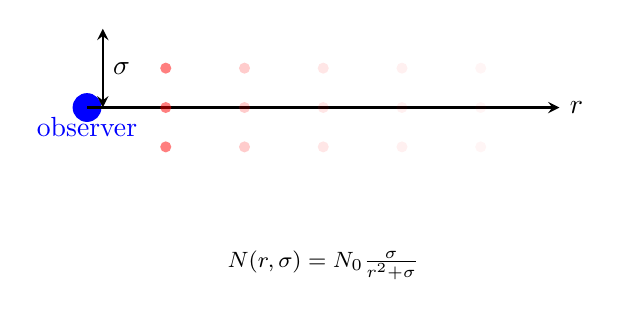
\begin{tikzpicture}[scale=1.0,>=stealth]
        \filldraw[blue] (0,0) circle (5pt) node[below] {observer};
        \draw[<->, thick] (0.2,0) -- (0.2,1.0) node[midway, right] {$\sigma$};
        \draw[->, thick] (0,0) -- (6,0) node[right] {$r$};
        \foreach \x in {1,2,3,4,5} {
            \foreach \y in {-0.5,0,0.5} {
                \pgfmathsetmacro{\opacity}{1/(1+\x*\x)}
                \fill[red, opacity=\opacity] (\x,\y) circle (2pt);
            }
        }
        \node[font=\footnotesize] at (3,-2) {$N(r,\sigma)=N_0\frac{\sigma}{r^2+\sigma}$};
    \end{tikzpicture}
    \caption{Scale-dependent sampling model. The density of sampling points decreases as the distance $r$ grows and increases as the observer scale $\sigma$ grows.}
    \label{fig:dynamic_sampling}
\end{figure}

\begin{property}[The monotonicity of sampling]\label{prop:sampling_monotonicity}
\begin{enumerate}[label=(\roman*)]
    \item For fixed $\sigma > 0$, $R$ and $N$ are strictly decreasing functions of the distance $r$.
    \item For fixed $r \ge 0$, $R$ and $N$ are strictly increasing functions of the scale $\sigma$.
\end{enumerate}
\end{property}

\begin{proof}
(i)
\[
\frac{\partial R}{\partial r} = R_0 \sigma \cdot \frac{-2r}{(r^2 + \sigma)^2} < 0 \quad (r > 0).
\]
(ii)
\[
\frac{\partial R}{\partial \sigma} = R_0 \cdot \frac{r^2}{(r^2 + \sigma)^2} \ge 0.
\]
The same holds for $N$.
\end{proof}

\begin{theorem}[The invisibility criterion]\label{thm:invisibility_criterion}
A source is \textbf{completely invisible} to an observer if and only if $N(r, \sigma) < 1$. The visibility threshold distance is
\[
r_{\text{max}} = \sqrt{(N_0 - 1)\sigma}.
\]
\end{theorem}

\begin{proof}
Solving $N_0 \cdot \frac{\sigma}{r^2 + \sigma} < 1$ gives
\[
N_0\sigma < r^2+\sigma
\iff
r^2 > (N_0-1)\sigma
\iff
r > \sqrt{(N_0-1)\sigma}.
\]
Hence the threshold distance is $r_{\text{max}} = \sqrt{(N_0 - 1)\sigma}$.
\end{proof}

\begin{remark}[Relation to the three sampling parameters]\label{rem:dynamic_sampling_vs_three}
Scale-dependent sampling turns the three fixed parameters of \cref{rem:sampling_three_parameters} into functions of the state: the sampling interval $\Delta x\mapsto1/R(r,\sigma)$ becomes coarser as the distance grows and finer as the scale grows; the number of sampling points $M\mapsto N(r,\sigma)$ varies in the same direction; and the sampling duration accordingly becomes $T=N(r,\sigma)/R(r,\sigma)$. Hence the proposition `the observer scale determines the range of distinguishability' acquires a precise quantitative form within the sampling framework of this chapter: when $N(r,\sigma)<1$ no information whatever is distinguishable (\cref{thm:invisibility_criterion}), and when $R(r,\sigma)$ falls below twice the signal frequency aliasing occurs (Section \ref{sec:aliasing}).
\end{remark}

\section{Epicycle groups: rotational decomposition of periodic signals}\label{sec:epicycle_system}

This section introduces the \textbf{epicycle group} (epicycle system). It unifies the Fourier series, the discrete phase operator and the congruence angle as `the superposition of rotational components'.

\begin{definition}[A single epicycle]\label{def:epicycle}
An \textbf{epicycle} is the following mapping:
\[
e_{A,\omega,\phi}(t):=A\,e^{i(\omega t+\phi)},\qquad t\in\mathbb{R},
\]
where $A\ge0$ is called the \textbf{radius} (amplitude), $\omega\in\mathbb{R}$ the \textbf{angular velocity} (frequency), and $\phi\in\mathbb{R}/2\pi\mathbb{Z}$ the \textbf{initial phase}. If $A=0$, the epicycle degenerates to zero.
\end{definition}

\begin{definition}[Epicycle group]\label{def:epicycle_system}
Let the index set $J$ be at most countable. The family
\[
\mathcal{E}:=\{(A_j,\omega_j,\phi_j)\}_{j\in J}
\]
is called an \textbf{epicycle group} if the composite signal
\[
x_{\mathcal{E}}(t):=\sum_{j\in J}A_j e^{i(\omega_j t+\phi_j)}
\]
converges in the specified function space. If $J$ is finite, $\mathcal{E}$ is called a \textbf{finite epicycle group}. The set
\[
\Omega(\mathcal{E}):=\{\omega_j:j\in J\}
\]
is called the \textbf{frequency set}.
\end{definition}

\begin{proposition}[The group with periodic orbits of an epicycle group]\label{prop:epicycle_group_with_periodic_orbits}
Let $\mathcal{E}=\{(A_j,\omega_j,\phi_j)\}_{j\in J}$ be a non-zero epicycle group such that $x_{\mathcal{E}}$ is non-constant. If the frequency set $\Omega(\mathcal{E})$ generates a discrete subgroup, write
\[
\omega_0:=\min\{\omega>0:\omega\in\textstyle\sum_j\mathbb{Z}\omega_j\}=\gcd\{\omega_j\ne0\}
\]
(that is, all $\omega_j/\omega_0\in\mathbb{Z}$); then $x_{\mathcal{E}}$ has period $T_x=2\pi/\lvert\omega_0\rvert$, and its group with periodic orbits is
\[
\operatorname{Group}_{\mathrm{period}}(x_{\mathcal{E}})=T_x\mathbb{Z}.
\]
The least positive period is $2\pi/\lvert\omega_0\rvert$ (an integer fraction of it when $\omega_0\notin\Omega$); when all $\omega_k=0$ there is no least positive period.

If the subgroup generated by $\Omega(\mathcal{E})$ in $\mathbb{R}$ is not discrete, then in general $x_{\mathcal{E}}$ has no non-trivial period.
\end{proposition}

\begin{proof}
If $\omega_j=k_j\omega_0$ with $k_j\in\mathbb{Z}$, then
\[
x_{\mathcal{E}}(t+T_x)=\sum_j A_j e^{i(k_j\omega_0(t+2\pi/\omega_0)+\phi_j)}
=\sum_j A_j e^{i(k_j\omega_0 t+\phi_j+2\pi k_j)}
=x_{\mathcal{E}}(t).
\]
Hence $T_x$ is a period. The least positive period is determined by the greatest common divisor $\omega_0=\gcd\{\omega_j\ne0\}$ of the non-zero frequencies: the least positive period is $2\pi/\lvert\omega_0\rvert$ (an integer fraction of it when $\omega_0\notin\Omega$); when all $\omega_k=0$ there is no least positive period. If the generated subgroup is not discrete, then the set of all non-zero periods has no least positive generator, and usually $\operatorname{Group}_{\mathrm{period}}(x_{\mathcal{E}})=\{0\}$.
\end{proof}

\begin{proposition}[Sampling and commensurability of epicycle groups]\label{prop:epicycle_sampling_commensurability}
Let the epicycle group $\mathcal{E}$ have frequency set $\Omega$, let the sampling interval be $\Delta x>0$, and let the sampling sequence be
\[
f(n)=x_{\mathcal{E}}(n\Delta x)=\sum_j A_j e^{i(\omega_j n\Delta x+\phi_j)}.
\]
If there exists $\omega_0>0$ with all $\omega_j/\omega_0\in\mathbb{Z}$, and the normalised period ratio $\rho=2\pi/(\omega_0\Delta x)$ is rational, then $f$ is a discrete periodic sequence; if $\rho\notin\mathbb{Q}$, then $f$ is aperiodic.
\end{proposition}

\begin{proof}
By Proposition \ref{prop:epicycle_group_with_periodic_orbits}, the period of the continuous signal is $T_x=2\pi/\omega_0$. Substituting into Proposition \ref{prop:commensurability_periodicity_parallel} gives the result.
\end{proof}

\begin{figure}[htbp]
\centering
\begin{tikzpicture}[>=Stealth, thick, scale=1.0]
% first-level epicycle
\draw[gray!50] (0,0) circle (1.6);
\draw[->, blue, very thick] (0,0) -- (1.6,0);
\node[blue, above, font=\footnotesize] at (0.8,0.1) {$A_1 e^{i\omega_1 t}$};
% second-level epicycle (centre at the endpoint of the first circle)
\draw[gray!50] (1.6,0) circle (0.7);
\draw[->, red, very thick] (1.6,0) -- (2.1,0.5);
\node[red, above right, font=\footnotesize] at (1.9,0.6) {$A_2 e^{i\omega_2 t}$};
% third-level epicycle
\draw[gray!50] (2.1,0.5) circle (0.3);
\fill (2.35,0.65) circle (1.5pt);
% explanation
\node[align=center, font=\small] at (0,-2.8) {Epicycle group: the geometric superposition of the periodic signal $x_{\mathcal{E}}(t)=\sum_j A_j e^{i(\omega_j t+\phi_j)}$};
\end{tikzpicture}
\caption{Epicycle group: the geometric realisation of the Fourier series. Each component is a uniformly rotating circle, and the final position of the moving point is the sum of the component vectors.}
\label{fig:epicycle_system}
\end{figure}

\begin{example}[A Fourier series is an epicycle group]\label{ex:fourier_epicycle}
The continuous periodic function $x(t)=\sum_{k\in\mathbb{Z}}c_k e^{i2\pi kt/T_x}$ corresponds to the epicycle group
\[
\mathcal{E}=\{(|c_k|,\ 2\pi k/T_x,\ \arg c_k)\}_{k\in\mathbb{Z}}.
\]
Hence the Fourier series expansion may be understood geometrically as: a family of epicycles whose angular velocities are integer multiples of the fundamental frequency superpose into the original periodic signal.
\end{example}

\begin{example}[The discrete Fourier transform is a finite epicycle group]\label{ex:dft_epicycle}
The DFT of a discrete periodic sequence $f:\mathbb{Z}/T_0\mathbb{Z}\to\mathbb{C}$ of length $T_0$,
\[
\hat f(k)=\sum_{n=0}^{T_0-1}f(n)e^{-i2\pi kn/T_0}
\]
decomposes $f$ into the finite epicycle group
\[
\mathcal{E}_f=\left\{\left(\frac{|\hat f(k)|}{T_0},\ \frac{2\pi k}{T_0},\ \arg \hat f(k)\right)\right\}_{k=0}^{T_0-1}.
\]
This is exactly the geometric interpretation of the discrete phase operator $\mathcal{O}_k^{(T_0)}=e^{i2\pi k/T_0}$ of this chapter.
\end{example}

\begin{remark}[Epicycle groups and congruence angles]\label{rem:epicycle_congruence}
The phase of each component of an epicycle group over a subperiod $T$ is precisely the congruence angle
\[
\langle \omega_j t+\phi_j\rangle_T
=\omega_j t+\phi_j\bmod \frac{2\pi}{T}.
\]
Hence a multi-period joint problem may be regarded as: an epicycle group has to close simultaneously over several subperiods. Intercalation is the adjustment of the observation window so that these congruence-angle errors are pressed down simultaneously.
\end{remark}

\begin{table}[htbp]
    \centering
    \caption{Metric parameters and components of discrete sampling approximation}
    \label{tab:discrete_period_parameters}
    \small
    \renewcommand{\arraystretch}{1.05}
    \begin{tabular}{>{\raggedright\arraybackslash\hspace{0pt}}p{2.4cm}>
                    {\raggedright\arraybackslash\hspace{0pt}}p{4.1cm}>
                    {\raggedright\arraybackslash\hspace{0pt}}p{4.1cm}>
                    {\raggedright\arraybackslash\hspace{0pt}}p{3.2cm}}
        \toprule
        Parameter & Definition & Time-domain meaning & Frequency-domain meaning \\
        \midrule
        Sampling interval $\Delta x$ & spacing of adjacent sampling points & time resolution & upper limit of distinguishability $\omega_N=\pi/\Delta x$ \\
        Sampling rate $\nu_s$ & $1/\Delta x$ & density of sampling points & the scale of the aliasing criterion \\
        Sampling duration $T$ & $M\Delta x$ & record length & frequency resolution $\Delta\omega=2\pi/T$ \\
        Period ratio $\rho$ & $T_x/\Delta x$ & sampling points in one period & position of the harmonic lattice \\
        Offset $\delta$ & $\|M\rho\|_{\mathbb{Z}}$ & deviation of the number of periods in the window & leakage strength \\
        Fundamental period $T_0$ & generator of $\operatorname{Group}_{\mathrm{period}}(f)$ & repetition length of the sequence & frequency-domain lattice spacing $2\pi/T_0$ \\
        Epicycle group $\mathcal{E}$ & $\{(A_j,\omega_j,\phi_j)\}$ & superposition of rotational components & set of Fourier modes \\
        Congruence angle $\langle\theta\rangle_T$ & $\theta\bmod 2\pi/T$ & phase modulo a subperiod & position of the spectral line on the subperiod \\
        Congruence-angle non-closure $\delta_T$ & $\frac{2\pi}{T}\|M\rho\|_{\mathbb{Z},T}$ & phase deviation on the subperiod & leakage strength on the subperiod \\
        \bottomrule
    \end{tabular}
\end{table}

\section{Finite windows, the Dirichlet kernel and spectral leakage}\label{sec:window_dirichlet}

This section gives the complete mechanism of spectral leakage. The conclusion is: \textbf{the root of leakage is that the number of periods inside the window is not an integer}; its mathematical carrier is the sidelobes of the Dirichlet kernel. Seen from the epicycle group, leakage is the superposition of sidelobes caused by the phase of each epicycle failing to close at the endpoints of the window.

\begin{definition}[Spectral leakage]\label{def:spectral_leakage}
Let the (true) spectrum of $x$ be $\hat x$. Suppose only a finite record of length $T=M\Delta x$,
\[
x_T(t):=x(t)\,\mathbf{1}_{[0,T)}(t),
\]
is observed, and its samples are subjected to a DFT. If $\hat x_T$ exhibits non-zero energy outside the spectral support of $\hat x$, then \textbf{spectral leakage} is said to occur. The amount of leakage is measured by the proportion of energy outside the main lobe,
\[
\eta:=\frac{\displaystyle\sum_{k\notin K_{\text{main lobe}}}|\hat f(k)|^2}{\displaystyle\sum_{k}|\hat f(k)|^2}
\]
where $K_{\text{main lobe}}$ is the set of frequency points covered by the main lobe (Definition \ref{def:mainlobe_sidelobe_parallel}).
\end{definition}

\begin{definition}[Dirichlet kernel]\label{def:dirichlet_kernel_parallel}
For an integer $M\ge0$ define the function
\[
D_M(\theta):=\sum_{m=-M}^{M}e^{im\theta},\qquad \theta\in\mathbb{R},
\]
called the \textbf{Dirichlet kernel} (also the Dirichlet function). Correspondingly, the normalised spectrum of the rectangular window of length $T$ is called the \textbf{window kernel}:
\[
W_T(\omega):=\frac{1}{T}\sum_{n=0}^{T-1}e^{-in\omega}
=\frac{e^{-i(T-1)\omega/2}}{T}\cdot\frac{\sin(T\omega/2)}{\sin(\omega/2)}
=\frac{e^{-i(T-1)\omega/2}}{T}\,D_{T-1}(\omega),
\]
whose modulus $|W_T(\omega)|=\frac{1}{T}\big|\frac{\sin(T\omega/2)}{\sin(\omega/2)}\big|$ depends only on the frequency.
\end{definition}

\begin{lemma}[Closed form of the Dirichlet kernel]\label{lem:dirichlet_kernel_closed_form}
For every $\theta\notin2\pi\mathbb{Z}$,
\[
D_M(\theta)=\frac{\sin\big((M+\tfrac12)\theta\big)}{\sin(\theta/2)},
\]
and $D_M(0)=2M+1$. In particular $|D_M(\theta)|\le\dfrac{1}{|\sin(\theta/2)|}$.
\end{lemma}

\begin{proof}
Multiplying $D_M(\theta)$ by $e^{-iM\theta}$ gives the geometric series
\[
\sum_{r=0}^{2M}e^{ir\theta}=\frac{e^{i(2M+1)\theta}-1}{e^{i\theta}-1}
=\frac{e^{i2M\theta}-e^{-i\theta}}{1-e^{-i\theta}} ,
\]
and substituting $1-e^{i\theta}=-2ie^{i\theta/2}\sin(\theta/2)$ and taking moduli gives the closed form; $D_M(0)=2M+1$ follows directly from the definition.
\end{proof}

\begin{figure}[htbp]
\centering
\begin{tikzpicture}[>=Stealth, thick, scale=1.0]
\draw[->] (-6.5,0) -- (6.5,0) node[right] {$\omega$};
\draw[->] (0,-0.5) -- (0,3.2) node[above] {$|W_T(\omega)|$};
\draw[blue, very thick, domain=-6.3:6.3, samples=500]
  plot (\x, {abs(sin(deg(2.5*\x)))/(2.5*abs(sin(deg(\x/2)))+0.0001)});
% main-lobe annotation
\draw[dashed, red] (-1.256,0) -- (-1.256,2.6);
\draw[dashed, red] (1.256,0) -- (1.256,2.6);
\draw[<->, red, thick] (-1.256,2.8) -- (1.256,2.8);
\node[red, above, font=\footnotesize] at (0,2.85) {main lobe};
% first sidelobe
\draw[<-, orange, thick] (2.0,0.9) -- (2.6,1.6);
\node[orange, right, font=\footnotesize] at (2.65,1.65) {first sidelobe $-13$ dB};
\node[align=center, font=\small] at (0,-1.6) {Window kernel $|W_T(\omega)|$ of the rectangular window: main-lobe width $4\pi/T$, sidelobes decaying as $|\omega|^{-1}$};
\end{tikzpicture}
\caption{Dirichlet kernel/window kernel of the rectangular window: main-lobe and sidelobe structure. The main-lobe width is $4\pi/T$, the first sidelobe is about $-13$ dB, and the sidelobe envelope decays as $|\omega|^{-1}$.}
\label{fig:dirichlet_kernel}
\end{figure}

\begin{lemma}[Orthogonality of the window kernel and the position of the main lobe]\label{lem:window_kernel_orthogonality_parallel}
We retain Definition \ref{def:dirichlet_kernel_parallel}. Then
\[
W_T\Big(\frac{2\pi k}{T}\Big)=\begin{cases}1, & k\equiv0\ (\mathrm{mod}\ T),\\[2pt]0, & \text{other integers }k,\end{cases}
\qquad
\sum_{n=0}^{T-1}e^{-i2\pi kn/T}=T\,\delta_{k,0\bmod T}.
\]
Moreover $|W_T(\omega)|$ attains its maximum $1$ at $\omega=0$ and first vanishes at $\omega=\pm2\pi/T$.
\end{lemma}

\begin{proof}
For $k\equiv0$ the sum is $T$; for $k\not\equiv0$ the ratio of the geometric series is $e^{-i2\pi k/T}\ne1$, and the sum is $\frac{1-e^{-i2\pi k}}{1-e^{-i2\pi k/T}}=0$. The maximum and the zeros are given by the numerator $\sin(T\omega/2)$ of Lemma \ref{lem:dirichlet_kernel_closed_form}, which vanishes at $\omega=2\pi j/T$ and attains its largest modulus near $\omega=0$.
\end{proof}

\begin{proposition}[Leakage formula for the truncation of a single tone]\label{prop:single_tone_leakage_parallel}
Let $f(n)=A e^{i(\omega_0 n+\phi)}$ ($A>0$, $\phi\in\mathbb{R}$), and take a DFT with a rectangular window of length $M$:
\[
\hat f(k)=\sum_{n=0}^{M-1}f(n)\,e^{-i2\pi kn/M},\qquad k=0,1,\dots,M-1.
\]
Then
\[
\hat f(k)=A e^{i\phi}\,e^{i\theta_k(M-1)/2}\,\frac{\sin(M\theta_k/2)}{\sin(\theta_k/2)},
\qquad \theta_k:=\omega_0-\frac{2\pi k}{M},
\]
and hence
\[
|\hat f(k)|=A\left|\frac{\sin(M\theta_k/2)}{\sin(\theta_k/2)}\right|.
\]
\end{proposition}

\begin{proof}
Substituting $f$ into the sum gives $\hat f(k)=Ae^{i\phi}\sum_{n=0}^{M-1}e^{i\theta_k n}$; applying the geometric-series summation formula $\sum_{n=0}^{M-1}e^{i\theta n}=e^{i\theta(M-1)/2}\frac{\sin(M\theta/2)}{\sin(\theta/2)}$ gives the result.
\end{proof}

\begin{theorem}[Leakage envelope and sidelobes]\label{thm:leakage_envelope_parallel}
Let $M\omega_0/(2\pi)=\nu+\delta$, where $\nu\in\mathbb{Z}$ and $\delta\in[-1/2,1/2]$ is the \textbf{offset} of the number of periods inside the window. Then
\begin{enumerate}[label=(\roman*)]
    \item the main lobe is located at $\nu$, with peak
    \[
    |\hat f(\nu)|=A\left|\frac{\sin(\pi\delta)}{\sin(\pi\delta/M)}\right|\xrightarrow[M\to\infty]{}A\,\frac{|\sin(\pi\delta)|}{\pi|\delta|}\cdot M;
    \]
    \item for $j\ne0$ we have $\theta_{\nu+j}=\frac{2\pi}{M}(\delta-j)$, so
    \[
    \frac{|\hat f(\nu+j)|}{|\hat f(\nu)|}
    =\frac{\big|\sin\big(\tfrac{\pi\delta}{M}\big)\big|}{\big|\sin\big(\tfrac{\pi(j-\delta)}{M}\big)\big|}
    \xrightarrow[M\to\infty]{}\frac{|\delta|}{|j-\delta|}=O\!\Big(\frac{1}{|j|}\Big),
    \]
    that is, \textbf{the sidelobe envelope decays reciprocally with the distance from the main frequency point}; the first sidelobe of the rectangular window is about $-13.3$ dB and decays as $|\omega|^{-1}$;
    \item if $\delta=0$ (the window contains exactly an integral number of periods), then $\hat f(k)=A M e^{i\phi}\delta_{k,\nu\bmod M}$, and \textbf{the leakage is zero};
    \item if $\delta\ne0$, then every frequency point carries non-zero energy, and the proportion of energy outside the \textbf{single peak frequency bin} is
    \[
    \eta(\delta)=1-\operatorname{sinc}^2(\delta)+O(M^{-1}),
    \qquad \operatorname{sinc}(u):=\frac{\sin(\pi u)}{\pi u},
    \]
    in particular $\eta(1/2)=1-4/\pi^2\approx0.595$, that is, in the worst case about $60\%$ of the energy lies outside the single peak frequency bin. For the main lobe of width $4\pi/T$ (Definition~\ref{def:mainlobe_sidelobe_parallel}) the corresponding value is $\eta_{\text{ML}}(1/2)=1-8/\pi^2\approx0.189$.
\end{enumerate}
\end{theorem}

\begin{proof}
(i) Substituting $k=\nu$ into Proposition \ref{prop:single_tone_leakage_parallel} and noting that $\theta_\nu=2\pi\delta/M$ gives $|\hat f(\nu)|=A\big|\frac{\sin(\pi\delta)}{\sin(\pi\delta/M)}\big|$; since $\sin(\pi\delta/M)\sim\pi\delta/M$, for $\delta\ne0$ this grows linearly in $M$ (the main-lobe peak is $O(M)$).

(ii) For $k=\nu+j$ ($j\ne0$) we have $\theta_k=\frac{2\pi}{M}(\delta-j)$, and substituting into Proposition \ref{prop:single_tone_leakage_parallel} gives $|\hat f(\nu+j)|=A\frac{|\sin(\pi(\delta-j))|}{|\sin(\pi(\delta-j)/M)|}=A\frac{|\sin(\pi\delta)|}{|\sin(\pi(j-\delta)/M)|}$; comparing with $|\hat f(\nu)|\approx AM|\sin(\pi\delta)|$ gives the stated ratio. The exact discrete value of the first sidelobe of the rectangular window differs slightly from the extremum of the continuous envelope, but its order of magnitude is $-13.3$ dB.

(iii) When $\delta=0$ we have $\theta_k=2\pi(\nu-k)/M$, and for $k\ne\nu\bmod M$ the numerator $\sin(\pi(\nu-k))=0$; hence only $k=\nu\bmod M$ is non-zero, with value $AMe^{i\phi}$.

(iv) By the discrete Parseval identity (Theorem \ref{thm:discrete_parseval_parallel}),
$\sum_{k=0}^{M-1}|\hat f(k)|^2=M\sum_{n=0}^{M-1}|f(n)|^2=M\cdot MA^2=M^2A^2$. The main-lobe energy is $|\hat f(\nu)|^2=A^2M^2\operatorname{sinc}^2(\delta)+O(M)$, so $\eta=1-\operatorname{sinc}^2(\delta)+O(M^{-1})$; for $|\delta|=1/2$ we have $\operatorname{sinc}(1/2)=2/\pi$, giving $\eta=1-4/\pi^2\approx0.595$.
\end{proof}

\begin{figure}[htbp]
\centering
\begin{tikzpicture}[>=Stealth, thick, scale=1.0]
\draw[->] (-0.3,0) -- (8.5,0) node[right] {frequency point $k$};
\draw[->] (0,-0.3) -- (0,2.8) node[above] {$|\hat f(k)|$};
% near the main lobe
\foreach \k in {0,1,...,16} {
  \pgfmathsetmacro{\x}{\k*0.5}
  \pgfmathsetmacro{\y}{abs(sin(deg(3.14159*(0.3+0.05*\k))))/(3.14159*abs(0.3+0.05*\k)+0.0001)}
  \pgfmathsetmacro{\yn}{\y>2.6?2.6:\y}
  \fill[blue] (\x,\yn) circle (2pt);
}
% highlight the energy outside the main lobe
\draw[red, thick, dashed] (1.5,0) -- (1.5,2.6);
\node[red, above, font=\footnotesize] at (1.5,2.6) {main lobe};
\draw[<-, orange, thick] (4.0,0.9) -- (5.0,1.8);
\node[orange, right, font=\footnotesize] at (5.05,1.85) {sidelobes (leaked energy)};
\node[align=center, font=\small] at (4.2,-1.4) {Leakage distribution for offset $\delta=0.3$: $\eta=1-\operatorname{sinc}^2(0.3)\approx0.088$};
\end{tikzpicture}
\caption{Energy distribution of spectral leakage: the main lobe is concentrated near the true frequency point, whilst the sidelobes scatter the leaked energy over all frequency points. The larger the offset $\delta$, the stronger the leakage.}
\label{fig:spectral_leakage}
\end{figure}

\begin{definition}[Main lobe and sidelobes]\label{def:mainlobe_sidelobe_parallel}
Let the zeros of the window kernel $|W_T(\omega)|$ on $\omega>0$ be $\omega_1<\omega_2<\cdots$ in order. The envelope on $[-\omega_1,\omega_1]$ is called the \textbf{main lobe}, and its \textbf{main-lobe width} is $2\omega_1$; the envelope on each interval $(\omega_j,\omega_{j+1})$ is called a \textbf{sidelobe}, its maximum is called the \textbf{sidelobe peak}, and the overall rate of decay of the sidelobe peaks with $j$ is called the \textbf{sidelobe decay rate}. For the rectangular window, $\omega_j=2\pi j/T$, the main-lobe width is $4\pi/T$, the first sidelobe peak is about $-13.3$ dB, and the sidelobe envelope decays as $|\omega|^{-1}$.
\end{definition}

\begin{corollary}[Integral windows have no leakage]\label{cor:integer_window_no_leakage}
Let $f(n)=Ae^{i(\omega_0 n+\phi)}$ with $\omega_0=2\pi m/T$ ($m\in\mathbb{Z}$); then the DFT with a rectangular window of length $T$ satisfies $\hat f(k)=ATe^{i\phi}\delta_{k,m\bmod T}$: \textbf{when the window contains exactly an integral number of periods, the discrete spectrum has only one spectral line and the leakage is zero}.
\end{corollary}

\begin{corollary}[Non-integral windows must leak]\label{cor:noninteger_window_leakage}
Let $\omega_0\notin\frac{2\pi}{T}\mathbb{Z}$. Then $\hat f(k)\ne0$ for all $k=0,\dots,T-1$, and the proportion of leaked energy is given by Theorem \ref{thm:leakage_envelope_parallel}(iv).
\end{corollary}

\begin{proposition}[Phase characterisation of leakage]\label{prop:leakage_phase_characterisation}
In the notation of Proposition \ref{prop:single_tone_leakage_parallel}, at non-zero points the amplitude ratio of adjacent frequency points,
\[
\frac{|\hat f(k+1)|}{|\hat f(k)|}=\left|\frac{\sin\big(\tfrac{\pi}{M}(k+1-\nu-\delta)\big)}{\sin\big(\tfrac{\pi}{M}(k-\nu-\delta)\big)}\right|
\]
depends only on $k-\nu$ and the offset $\delta$, whilst the phase difference
\[
\arg\frac{\hat f(k+1)}{\hat f(k)}=-\frac{\pi(M-1)}{M}+\varepsilon_k,\qquad
\varepsilon_k\in\{0,\pi\},
\]
is independent of $k$, where $\varepsilon_k=\pi$ if and only if the two frequency points lie on opposite sides of the main-lobe peak (that is, the pair of frequency points straddles $\nu+\delta$). Hence: \textbf{the pattern of values of the phase difference locates the main lobe, and the amplitude ratio inverts the offset}---this is precisely the principle of \textbf{two-spectral-line interpolation} and of \textbf{phase-difference frequency estimation}.
\end{proposition}

\begin{proof}
By the closed form of Proposition \ref{prop:single_tone_leakage_parallel},
$\hat f(k)=Ae^{i\phi}e^{i\theta_k(M-1)/2}\frac{\sin(M\theta_k/2)}{\sin(\theta_k/2)}$. The first formula follows for the amplitude. The phase consists of the linear term $\theta_k(M-1)/2$ and the sign of the sine factor: $\theta_{k+1}-\theta_k=-2\pi/M$ gives the adjacent phase difference $-\pi(M-1)/M$, whilst $\sin(M\theta_k/2)=\sin(\pi(k-\nu-\delta))$ has opposite signs at adjacent frequency points if and only if those two points lie on opposite sides of the zero $\nu+\delta$, contributing an additional phase $\pi$; in all other cases the signs agree. Hence the phase difference takes only two possible values, independently of $k$, and the position at which it flips directly gives the continuous position $\nu+\delta$ of the main lobe.
\end{proof}

\begin{proposition}[Congruence-angle characterisation of leakage]\label{prop:leakage_congruence_angle}
Let $f(n)=Ae^{i\omega_0 n}$ with $\omega_0=2\pi\rho$ and window length $M$. Then the single-period leakage proportion may be written as
\[
\eta(M)=1-\operatorname{sinc}^2\!\big(\|M\rho\|_{\mathbb{Z}}\big)+O(M^{-1}),
\]
where $\|M\rho\|_{\mathbb{Z}}$ is the offset of the number of periods inside the window. If a subperiod $T$ is introduced, then when $T\mid M\rho$ the congruence-angle non-closure over that subperiod is $\delta_T=0$, and the leakage is closed in the sense of that subperiod.
\end{proposition}

\begin{proof}
This follows from Theorem \ref{thm:leakage_envelope_parallel}(iv); the assertion about the subperiod follows directly from Definition \ref{def:congruence_angle_misclosure} and $T\mid M\rho$.
\end{proof}

\begin{example}[Numerical magnitude of leakage]\label{ex:rectangular_leakage_numeric}
Take $f(n)=e^{i2\pi(0.25+0.5/M)n}$ (that is, $\delta=1/2$, the main lobe falling exactly between two frequency points) and $M=16$. By Theorem \ref{thm:leakage_envelope_parallel}(iv) the leakage proportion is $\eta\approx0.595$, that is, about $60\%$ of the energy is distributed outside the main lobe; the two bins of the main lobe take about $40.7\%$ each, so that the main lobe (two bins) holds about $81\%$, and the remaining sidelobes about $19\%$ in total. If the window length is changed to $M=20$ and $\omega_0=2\pi\cdot7/20$ is taken ($\delta=0$), then all the energy is concentrated in a single spectral line and $\eta=0$.
\end{example}

\begin{remark}[Inevitability and controllability of leakage]\label{rem:leakage_inevitability}
By Corollary \ref{cor:noninteger_window_leakage}, as long as the number of periods inside the window is not an integer, leakage necessarily occurs---this is the price of `finite observation' and is independent of the sampling rate (the latter determines aliasing). But Theorem \ref{thm:leakage_envelope_parallel}(iv) shows that the leakage strength \textbf{depends only on the offset} $\delta=\|M\rho\|_{\mathbb{Z}}$: as long as $\delta$ is pressed down, the leakage is small. This converts the problem of leakage control into a purely number-theoretic problem---\textbf{approximating the real period ratio optimally by an integral window length}---and this is precisely intercalation (Section \ref{sec:commensurability_intercalation}).
\end{remark}

\section{Aliasing: the price of the sampling rate}\label{sec:aliasing}

The preceding section showed that leakage is determined by the \textbf{sampling duration}. This section shows that the other class of error---\textbf{aliasing}---is determined by the \textbf{sampling rate}; the two are independent and must be handled separately.

\begin{definition}[Aliasing]\label{def:aliasing_parallel}
Let the angular sampling rate be $\omega_s=2\pi/\Delta x$. Two angular frequencies $\omega,\omega'\in\mathbb{R}$ are said to be \textbf{aliased} if
\[
\omega'\equiv\omega\pmod{\omega_s},
\qquad\text{that is,}\qquad
\omega'=\omega+m\omega_s,\quad m\in\mathbb{Z}.
\]
The functions $e^{i\omega t}$ and $e^{i\omega' t}$ take exactly the same values on the sampling lattice $\Lambda_{\Delta x}$, so the two are \textbf{indistinguishable} after sampling; this phenomenon is called \textbf{aliasing} (frequency folding).
\end{definition}

\begin{proposition}[The folding map]\label{prop:aliasing_frequency_map_parallel}
Define the folding map
\[
\mathcal{A}_{\omega_s}:\mathbb{R}\to\Big(-\frac{\omega_s}{2},\frac{\omega_s}{2}\Big],\qquad
\mathcal{A}_{\omega_s}(\omega):=\omega-m\,\omega_s,
\quad m:=\Big\lfloor\frac{\omega}{\omega_s}+\frac12\Big\rfloor .
\]
Then
\begin{enumerate}[label=(\roman*)]
    \item $\mathcal{A}_{\omega_s}(\omega)$ is aliased with $\omega$, and $|\omega-\mathcal{A}_{\omega_s}(\omega)|\le\omega_s/2$;
    \item $\mathcal{A}_{\omega_s}$ is surjective but not injective, and each preimage class is exactly $\{\omega+m\omega_s\}_{m\in\mathbb{Z}}$;
    \item $\mathcal{A}_{\omega_s}$ is a translation on each Nyquist band $\big(\tfrac{2k-1}{2}\omega_s,\tfrac{2k+1}{2}\omega_s\big]$, and on the $k$-th band it is a reflection composed with a translation ($k$ alternating in parity).
\end{enumerate}
\end{proposition}

\begin{proof}
(i) By definition $\omega-\mathcal{A}(\omega)=m\omega_s\in\omega_s\mathbb{Z}$, hence aliasing; moreover $m$ is the nearest integer, so $|m-\omega/\omega_s|\le1/2$, that is, $|\omega-\mathcal{A}(\omega)|\le\omega_s/2$. (ii) For every $\eta\in(-\omega_s/2,\omega_s/2]$ we have $\eta=\mathcal{A}(\eta)$, so the map is surjective; if $\mathcal{A}(\omega)=\mathcal{A}(\omega')$ then $\omega-\omega'\in\omega_s\mathbb{Z}$, so each preimage class is an arithmetic progression. (iii) Within a band $m$ is constant, so $\mathcal{A}(\omega)=\omega-k\omega_s$ is a translation; at the band boundaries $m$ jumps once, so the images on two adjacent bands have opposite directions.
\end{proof}

\begin{figure}[htbp]
\centering
\begin{tikzpicture}[>=Stealth, thick, scale=0.9]
\draw[->] (-4.5,0) -- (4.5,0) node[right] {$\omega$};
\draw[->] (0,-2.5) -- (0,1.5) node[above] {$\mathcal{A}(\omega)$};
% Nyquist bands
\draw[dashed, gray] (-3.14,0) -- (-3.14,-2.4);
\draw[dashed, gray] (-1.57,0) -- (-1.57,-2.4);
\draw[dashed, gray] (1.57,0) -- (1.57,-2.4);
\draw[dashed, gray] (3.14,0) -- (3.14,-2.4);
\node[font=\footnotesize] at (-3.14,-2.55) {$-2\pi$};
\node[font=\footnotesize] at (-1.57,-2.55) {$-\pi$};
\node[font=\footnotesize] at (0,-2.55) {$0$};
\node[font=\footnotesize] at (1.57,-2.55) {$\pi$};
\node[font=\footnotesize] at (3.14,-2.55) {$2\pi$};
% folding curve
\draw[blue, very thick] (-4.5,0) -- (-3.14,0) -- (-3.14,-1.57) -- (-1.57,-1.57) -- (-1.57,0) -- (0,0) -- (0,0) -- (1.57,0) -- (1.57,-1.57) -- (3.14,-1.57) -- (3.14,0) -- (4.5,0);
\node[align=center, font=\small] at (0,-3.6) {Folding map $\mathcal{A}_{\omega_s}(\omega)$: all Nyquist bands are folded into $(-\pi,\pi]$};
\end{tikzpicture}
\caption{The folding map of aliasing: each Nyquist band on the frequency axis (of width $\omega_s=2\pi$) is folded into the fundamental interval $(-\pi,\pi]$. All aliased frequencies are indistinguishable within that interval.}
\label{fig:aliasing_folding}
\end{figure}

\begin{theorem}[Nyquist--Shannon sampling theorem]\label{thm:nyquist_shannon_parallel}
Let $x\in L^2(\mathbb{R})$ be continuous and let its Fourier transform $\hat x$ satisfy the support condition
\[
\operatorname{supp}\hat x\subset(-\omega_N,\omega_N),\qquad \omega_N=\frac{\pi}{\Delta x},
\]
then $x$ is uniquely reconstructed from its samples $\{x(n\Delta x)\}_{n\in\mathbb{Z}}$:
\[
x(t)=\sum_{n\in\mathbb{Z}}x(n\Delta x)\,\operatorname{sinc}\!\Big(\frac{t-n\Delta x}{\Delta x}\Big),
\qquad
\operatorname{sinc}(u):=\frac{\sin(\pi u)}{\pi u},
\]
and the series converges in $L^2$ and in the uniform norm.
\end{theorem}

\begin{proof}
By the band-limited condition, the terms of the frequency periodisation
\[
P(\omega):=\frac{1}{\Delta x}\sum_{m\in\mathbb{Z}}\hat x\Big(\omega+\frac{2\pi m}{\Delta x}\Big)
\]
have mutually non-overlapping supports, so $P$ agrees with $\hat x/\Delta x$ on $(-\omega_N,\omega_N)$. On the other hand, $P$ is the discrete-time Fourier transform (of period $2\pi/\Delta x$) of the sampling sequence $\{x(n\Delta x)\}$. Restricting $P$ to $(-\omega_N,\omega_N)$ and setting it to zero elsewhere, and multiplying by the rectangular window $W$ (whose inverse transform is $\operatorname{sinc}(t/\Delta x)/\Delta x$), gives the reconstruction formula; the convergence of the series follows from $x\in L^2$ and the orthogonality of $\operatorname{sinc}$.
\end{proof}

\begin{lemma}[Poisson-summation proof of the sampling theorem]\label{lem:poisson_summation_sampling}
The spectrum of the sampling sequence can be written, using the Poisson summation formula, as
\[
\sum_{n\in\mathbb{Z}}x(n\Delta x)e^{-i\omega n\Delta x}
=\frac{1}{\Delta x}\sum_{m\in\mathbb{Z}}\hat x(\omega+2\pi m/\Delta x).
\]
\end{lemma}

\begin{proof}
By the inverse Fourier transform $x(n\Delta x)=\frac{1}{2\pi}\int\hat x(\omega')e^{in\Delta x\omega'}d\omega'$; substituting into the left-hand side gives
\[
\sum_n x(n\Delta x)e^{-i\omega n\Delta x}=\frac{1}{2\pi}\sum_n\int\hat x(\omega')e^{in\Delta x(\omega'-\omega)}d\omega'.
\]
Using the Poisson summation formula $\sum_ne^{in\Delta x\theta}=\frac{2\pi}{\Delta x}\sum_m\delta(\theta-2\pi m/\Delta x)$ and interchanging the sum and the integral gives the result.
\end{proof}

\begin{corollary}[Irreversibility of aliasing]\label{cor:aliasing_irreversibility_parallel}
Let $\omega\ne\omega'$ with $\omega'\equiv\omega\pmod{\omega_s}$. Then $\mathcal{S}_{\Delta x}e^{i\omega\cdot}=\mathcal{S}_{\Delta x}e^{i\omega'\cdot}$, so no algorithm that depends only on the samples can distinguish the two; the sampling operator is irreversible on each aliasing class. Anti-aliasing can only be carried out before it, that is, by \textbf{analogue low-pass filtering before sampling}.
\end{corollary}

\begin{definition}[Anti-aliasing filter]\label{def:anti_aliasing_filter}
Let the spectral support of the signal $x$ exceed the Nyquist frequency. An \textbf{anti-aliasing filter} is a low-pass filter $h$ with cut-off frequency $\omega_N$: before sampling one first forms the convolution $x_{\text{filt}}=h*x$ and then samples with spacing $\Delta x$. The filtered signal satisfies the band-limited condition, so that the sampling theorem applies.
\end{definition}

\begin{property}[Ideal properties of the anti-aliasing filter]\label{prop:anti_aliasing_ideal}
An ideal anti-aliasing filter equals a rectangular window in the frequency domain:
\[
\hat h(\omega)=\mathbf{1}_{(-\omega_N,\omega_N)}(\omega).
\]
Then the filtered signal is undistorted within the band and completely removed outside it, so that the sampling theorem holds and aliasing is strictly zero.
\end{property}

\begin{proof}
By the convolution theorem $\widehat{x_{\text{filt}}}=\hat h\hat x$, so $\operatorname{supp}\widehat{x_{\text{filt}}}\subseteq(-\omega_N,\omega_N)$, which satisfies the band-limited condition of the sampling theorem. Within the band $\hat h=1$ guarantees that the signal is unchanged.
\end{proof}

\begin{remark}[The difference between aliasing and leakage]\label{rem:aliasing_vs_leakage}
Aliasing and leakage are two independent sources of error, easily confused, and must be strictly distinguished:
\begin{enumerate}[label=(\roman*)]
    \item \textbf{Source}: aliasing comes from \textbf{discretisation} (finite sampling rate, $\Delta x>0$); leakage comes from \textbf{truncation} (finite sampling duration, $T<\infty$).
    \item \textbf{Mathematical mechanism}: aliasing is the \textbf{folding of frequency modulo $\omega_s$} (Proposition \ref{prop:aliasing_frequency_map_parallel}); leakage is the \textbf{convolutional spill-over} of the true spectrum with the window kernel (Theorem \ref{thm:leakage_envelope_parallel}).
    \item \textbf{Means of control}: aliasing is dealt with by raising $\nu_s$ or by a preposed anti-aliasing filter; leakage is dealt with by lengthening $T$ or by \textbf{intercalation} (Section \ref{sec:commensurability_intercalation}).
    \item \textbf{Reversibility}: aliasing is irreversible (Corollary \ref{cor:aliasing_irreversibility_parallel}); leakage is reversible---as long as the offset $\delta=0$, the leakage disappears completely (Corollary \ref{cor:integer_window_no_leakage}).
\end{enumerate}
\end{remark}

\begin{example}[A numerical example of aliasing]\label{ex:aliasing_numeric}
Take $\Delta x=1$ s (so $\omega_s=2\pi$ rad/s). The signals $x_1(t)=\cos(2\pi\cdot0.9\,t)$ and $x_2(t)=\cos(2\pi\cdot0.1\,t)$ have exactly the same samples:
\[
\cos(2\pi\cdot0.9\,n)=\cos(2\pi\cdot0.1\,n),\qquad n\in\mathbb{Z},
\]
because $0.9\equiv-0.1\pmod1$ and the cosine is an even function. In the spectrum the two lie at $0.9$ and $0.1$ cycles per second respectively, and after sampling both fall at $\pm0.1$ cycles per second. If only the samples are observed, it is impossible to decide whether the true frequency is $0.9$ or $0.1$---this is precisely the practical meaning of aliasing.
\end{example}

\section{Upper and lower approximation}\label{sec:bounded_approximation}

By Theorem \ref{thm:leakage_envelope_parallel}(iv), the leakage strength depends only on the offset $\delta=\|M\rho\|_{\mathbb{Z}}$. Hence leakage control is equivalent to: \textbf{approximating the real period ratio $\rho$ by an integral window length $M$}. This section establishes the two basic tools of this approximation---the upper approximation and the lower approximation---and gives the optimality of continued fractions.

\begin{definition}[Upper and lower approximation]\label{def:bounded_approximation_parallel}
Let $\rho>0$ and $M\in\mathbb{N}^+$. Define
\[
\begin{aligned}
\rho^{(-)}_M&:=\frac{\lfloor M\rho\rfloor}{M}\quad(\text{lower approximation}),\\
\rho^{(+)}_M&:=\frac{\lceil M\rho\rceil}{M}\quad(\text{upper approximation}),\\
\rho^{(\pm)}_M&:=\frac{\lfloor M\rho+\tfrac12\rfloor}{M}\quad(\text{balanced approximation}),
\end{aligned}
\]
and call $\delta_M:=\|M\rho\|_{\mathbb{Z}}:=\min_{m\in\mathbb{Z}}|M\rho-m|$ the \textbf{offset} of the window $M$.
\end{definition}

\begin{proposition}[Integrality inequalities]\label{prop:bounds_integrality}
For every $\rho>0$ and $M\in\mathbb{N}^+$,
\[
0\le M\rho-\lfloor M\rho\rfloor<1,\qquad 0\le\lceil M\rho\rceil-M\rho<1,\qquad
\lceil M\rho\rceil-\lfloor M\rho\rfloor\in\{0,1\},
\]
and $\delta_M=\min\{M\rho-\lfloor M\rho\rfloor,\ \lceil M\rho\rceil-M\rho\}\le1/2$.
\end{proposition}

\begin{proof}
The first two formulas follow from the definition of the integer part: $M\rho-1<\lfloor M\rho\rfloor\le M\rho\le\lceil M\rho\rceil<M\rho+1$; the third follows because the difference of the two is less than $2$ and is an integer. The expression for the offset follows because $\delta_M$ is the distance from $M\rho$ to the nearest integer, hence $\le1/2$.
\end{proof}

\begin{proposition}[Congruence-angle formulation of the upper and lower approximation]\label{prop:bounded_approx_congruence}
The upper approximation $\rho^{(+)}_M$ corresponds to a positive congruence-angle error and the lower approximation $\rho^{(-)}_M$ to a negative congruence-angle error:
\[
\rho^{(+)}_M-\rho=\frac{\delta_M^+}{M},\qquad
\rho-\rho^{(-)}_M=\frac{\delta_M^-}{M},
\]
where $\delta_M^\pm\ge0$ and $\delta_M^++\delta_M^-=\delta_M$. The balanced approximation $\rho^{(\pm)}_M$ makes the two equal.
\end{proposition}

\begin{proof}
This follows from Definition \ref{def:bounded_approximation_parallel} and Proposition \ref{prop:bounds_integrality}.
\end{proof}

\begin{theorem}[Upper and lower bounds for approximation error]\label{thm:intercalation_error_bound_parallel}
Let $\rho>0$ and $M\in\mathbb{N}^+$. Then
\begin{enumerate}[label=(\roman*)]
    \item \textbf{Sandwiching}: $\rho^{(-)}_M\le\rho\le\rho^{(+)}_M$, and the errors of the upper and lower approximation are respectively
    \[
    \rho-\rho^{(-)}_M=\frac{M\rho-\lfloor M\rho\rfloor}{M}<\frac1M,
    \qquad
    \rho^{(+)}_M-\rho=\frac{\lceil M\rho\rceil-M\rho}{M}<\frac1M;
    \]
    \item \textbf{Optimality of the balanced approximation}: $|\rho-\rho^{(\pm)}_M|=\delta_M/M\le\dfrac{1}{2M}$, and for fixed $M$ this is the smallest error among all approximations by `integer numerator $/$ denominator $M$';
    \item \textbf{Intercalation formulation}: let $E_M\subseteq\{1,\dots,M\}$ be the set of intercalation positions chosen according to the balanced scheme (that is, the $n$-th position is intercalated if and only if $\lfloor(n+1)\rho\rfloor-\lfloor n\rho\rfloor=1$); then
    \[
    \big||E_M|-M\rho\big|<1,
    \]
    that is, the difference between the number of intercalations and the ideal value $M\rho$ is less than one unit.
\end{enumerate}
\end{theorem}

\begin{proof}
(i) Dividing $\lfloor M\rho\rfloor\le M\rho\le\lceil M\rho\rceil$ by $M$ gives the sandwiching; the error formulas follow from the margin below $1$ in Proposition \ref{prop:bounds_integrality}.

(ii) The numerator of $\rho^{(\pm)}_M=\frac{\lfloor M\rho+1/2\rfloor}{M}$ is the nearest integer to $M\rho$, so $|\rho-\rho^{(\pm)}_M|=\delta_M/M$; for any integer $p$ we have $|\rho-p/M|=|M\rho-p|/M\ge\delta_M/M$, so minimality holds.

(iii) Write $N_M:=|E_M|$. Summing step by step from the definition of the balanced sequence gives
\[
N_M=\sum_{n=1}^{M}\big(\lfloor(n+1)\rho\rfloor-\lfloor n\rho\rfloor\big)=\lfloor(M+1)\rho\rfloor-\lfloor\rho\rfloor,
\]
and on the other hand $\lfloor(M+1)\rho\rfloor-\lfloor\rho\rfloor=M\rho+\{(M+1)\rho\}-\{\rho\}$ (where $\{\cdot\}$ denotes the fractional part), and since $0\le\{(M+1)\rho\}<1$ whilst $0\le\{\rho\}<1$ we have $\{(M+1)\rho\}-\{\rho\}<1$, and this difference also exceeds $-1$, so $|N_M-M\rho|<1$.
\end{proof}

\begin{figure}[htbp]
\centering
\begin{tikzpicture}[>=Stealth, thick, scale=0.9]
\draw[->] (-0.3,0) -- (7.5,0) node[right] {$M$};
\draw[->] (0,-0.3) -- (0,2.6) node[above] {$\rho^{(\cdot)}_M$};
\draw[dashed, red, thick] (0,1.5) -- (7.2,1.5);
\node[red, above, font=\footnotesize] at (7.2,1.5) {$\rho$};
% upper approximation
\foreach \M in {1,2,...,7} {
  \pgfmathsetmacro{\x}{\M*0.9}
  \pgfmathsetmacro{\yup}{ceil(1.5*\M)/\M}
  \pgfmathsetmacro{\ydn}{floor(1.5*\M)/\M}
  \fill[blue] (\x,\yup) circle (2pt);
  \fill[green!60!black] (\x,\ydn) circle (2pt);
}
\node[blue, above, font=\footnotesize] at (3.2,2.1) {upper approximation $\rho^{(+)}_M$};
\node[green!60!black, below, font=\footnotesize] at (3.2,0.3) {lower approximation $\rho^{(-)}_M$};
\node[align=center, font=\small] at (3.7,-1.0) {The upper/lower approximations sandwich $\rho$ from both sides, with convergence rate $O(1/M)$};
\end{tikzpicture}
\caption{Upper approximation and lower approximation: the blue points sandwich the true value $\rho$ (red line) from above and the green points from below, both with error $O(1/M)$. The balanced approximation takes their midpoint, with error $O(1/(2M))$.}
\label{fig:bounded_approximation}
\end{figure}

\begin{proposition}[Convergence of the sandwich]\label{prop:sandwich_convergence_parallel}
For every $\rho>0$, the sequence $\rho^{(-)}_M$ is monotonically non-decreasing and $\rho^{(+)}_M$ is monotonically non-increasing; both converge to $\rho$, with convergence rate $O(1/M)$:
\[
0\le\rho-\rho^{(-)}_M<1/M,\qquad 0\le\rho^{(+)}_M-\rho<1/M,\qquad
\rho^{(-)}_M\le\rho^{(\pm)}_M\le\rho^{(+)}_M .
\]
\end{proposition}

\begin{proof}
Monotonicity is given by nested windows: for $M<M'$ we have $\lfloor M\rho\rfloor/M\le\lfloor M'\rho\rfloor/M'$ (obtained by cross-multiplication). Convergence follows directly from the bounds of Theorem \ref{thm:intercalation_error_bound_parallel}(i), and the sandwiching inequality follows because the three are of the same order.
\end{proof}

\begin{proposition}[Scaling of the error with the denominator]\label{prop:error_denominator_scaling_parallel}
Let $\rho\notin\mathbb{Q}$.
\begin{enumerate}[label=(\roman*)]
    \item For a general window $M$ the offset satisfies $\delta_M\le1/2$, so the approximation error is $O(1/M)$;
    \item if $M=q_k$ is taken (a continued-fraction denominator of $\rho$), then $\delta_{q_k}<1/q_{k+1}$, so the approximation error is $O(1/M^2)$, an \textbf{improvement by one order of magnitude} over a general window;
    \item for any window sequence $M_j\to\infty$, one cannot guarantee that $\delta_{M_j}\to0$; only the subsequence taken along continued-fraction denominators guarantees $\delta_{q_k}\to0$ with quadratic convergence.
\end{enumerate}
\end{proposition}

\begin{proof}
(i) By Proposition \ref{prop:bounds_integrality}. (ii) By $\delta_{q_k}=|q_k\rho-p_k|<1/q_{k+1}$ from Theorem \ref{thm:continued_fraction_best_approx_parallel}(ii), and since $q_{k+1}>q_k$ we have $\delta_{q_k}/q_k<1/(q_kq_{k+1})=O(q_k^{-2})$. (iii) Take $M_j$ such that $\{M_j\rho\}$ has a positive limit inferior; then $\delta_{M_j}$ does not tend to zero.
\end{proof}

\begin{theorem}[Best continued-fraction approximation]\label{thm:continued_fraction_best_approx_parallel}
Let the continued-fraction expansion of $\rho\notin\mathbb{Q}$ be
\[
\rho=[a_0;a_1,a_2,\dots],\qquad a_0\in\mathbb{Z},\ a_j\in\mathbb{N}^+\ (j\ge1),
\]
with convergents denoted $p_k/q_k$ ($p_k,q_k$ coprime, $q_k\to\infty$). Then
\begin{enumerate}[label=(\roman*)]
    \item \textbf{Error bound}: $\Big|\rho-\dfrac{p_k}{q_k}\Big|<\dfrac{1}{q_kq_{k+1}}<\dfrac{1}{q_k^2}$;
    \item \textbf{Best-approximation property}: if $0<q<q_{k+1}$ and $p\in\mathbb{Z}$, then $|q\rho-p|\ge|q_k\rho-p_k|$; that is, no rational number with denominator less than $q_{k+1}$ can be closer to $\rho$ than $p_k/q_k$;
    \item \textbf{Offset equivalence}: $\delta_{q_k}=|q_k\rho-p_k|$ is strictly decreasing, and $\dfrac{1}{q_k+q_{k+1}}<\delta_{q_k}<\dfrac{1}{q_{k+1}}$.
\end{enumerate}
\end{theorem}

\begin{proof}
(i) The classical identity for continued fractions,
\[
\rho-\frac{p_k}{q_k}=\frac{(-1)^k}{q_k\,(q_{k+1}+q_k\beta_{k+1})},\qquad \beta_{k+1}=[a_{k+1};a_{k+2},\dots]>0
\]
immediately gives $|\rho-p_k/q_k|<1/(q_kq_{k+1})$, and $q_{k+1}>q_k$ gives the second formula.

(ii) By Legendre's theorem: every rational number satisfying $|\rho-p/q|<1/(2q^2)$ must be a convergent; combining this with $q_{k+1}\le2q_k$ gives the conclusion.

(iii) From (i) and $\beta_{k+1}\ge a_{k+1}\ge1$ we obtain the lower bound $\delta_{q_k}>\frac{1}{q_k+q_{k+1}}$; the decreasing property follows because $\rho$ lies between $p_k/q_k$ and $p_{k+1}/q_{k+1}$ and the two errors have alternating signs.
\end{proof}

\begin{figure}[htbp]
\centering
\begin{tikzpicture}[>=Stealth, thick, scale=1.0]
\draw[->] (-0.3,0) -- (8.5,0) node[right] {$k$};
\draw[->] (0,-0.3) -- (0,3.0) node[above] {$\log_{10}\delta_{q_k}$};
% data points (schematic)
\foreach \k/\d in {1/0.4, 2/0.1, 3/0.05, 4/0.01, 5/0.003, 6/0.001, 7/0.0003} {
  \pgfmathsetmacro{\x}{\k*1.0}
  \pgfmathsetmacro{\y}{3+log10(\d)/3}
  \fill[blue] (\x,\y) circle (2.5pt);
}
\draw[blue, thick, dashed] (1,2.85) -- (7,0.6);
\node[blue, above, font=\footnotesize] at (5.5,1.5) {$\delta_{q_k}=O(1/q_{k+1})$};
\node[align=center, font=\small] at (4.2,-1.2) {The offset $\delta_{q_k}$ of the convergents of a continued fraction decreases as $1/q_{k+1}$, one order of magnitude faster than the $1/M$ of a general window};
\end{tikzpicture}
\caption{Optimal approximation by continued-fraction convergents: the offset $\delta_{q_k}$ decreases as $O(1/q_{k+1})$ as the denominator $q_k$ grows, that is, the leakage of the intercalation window decays as $O(q_k^{-2})$.}
\label{fig:continued_fraction_convergence}
\end{figure}

\begin{theorem}[Best intercalation]\label{thm:best_intercalation_parallel}
Let $\rho>0$ be the period ratio (the number of units in one period). The intercalation problem asks: to realise $\rho$ integrally within $M$ basic units. Then
\begin{enumerate}[label=(\roman*)]
    \item there exists a sequence of intercalation windows $\{M_k\}$ for which the error $|\rho-\rho^{(\pm)}_{M_k}|$ converges quadratically, that is, as $O(M_k^{-2})$;
    \item the optimal sequence of window lengths is exactly the sequence of continued-fraction denominators $\{q_k\}$: within $q_k$ units one takes $p_k$ intercalation units, the error is $\delta_{q_k}<1/q_{k+1}$, and (when $\rho\notin\mathbb{Q}$) no smaller window length attains the same accuracy;
    \item for each $k$ the sign of the error alternates: $p_k/q_k$ approaches $\rho$ alternately from above and below, so the upper approximation and the lower approximation need only be \textbf{used alternately} to attain optimality.
\end{enumerate}
\end{theorem}

\begin{proof}
The accuracy in (ii) is given by Theorem \ref{thm:continued_fraction_best_approx_parallel}(iii); optimality is the best-approximation property of (ii). (i) is obtained from (ii) by taking $M_k=q_k$. (iii) follows from the alternation of the convergents of a continued fraction.
\end{proof}

\begin{corollary}[Optimality of balanced intercalation]\label{cor:balanced_intercalation_optimal}
Let $\rho\notin\mathbb{Q}$ and $M=q_k$. The error of the balanced intercalation sequence satisfies
\[
\big||E_M|-M\rho\big|\le\delta_{q_k}<\frac1{q_{k+1}},
\]
that is, the deviation on this window is exactly $\delta_{q_k}$ and does not exceed the continued-fraction error bound $1/q_{k+1}$. Among all intercalation schemes with window length $M=q_k$ the distance between the number of intercalations $|E_M|$ and $M\rho$ cannot be smaller than $\delta_{q_k}$, so \textbf{balanced intercalation attains optimal accuracy on the shortest window}.
\end{corollary}

\begin{example}[Quantitative analysis of the 19-year 7-intercalation cycle]\label{ex:metonic_parallel}
Take the tropical year $T_x=365.2422$ days and the synodic month $T_{\mathrm{syn}}=29.530588$ days. Taking the `month' as the basic unit and the `year' as the period, the period ratio is
\[
\rho=\frac{T_x}{T_{\mathrm{syn}}}\approx12.368266 .
\]
Its continued-fraction expansion is $[12;2,1,2,1,1,16,\dots]$, with convergents
\[
\frac{12}{1},\ \frac{25}{2},\ \frac{37}{3},\ \frac{99}{8},\ \frac{136}{11},\ \frac{235}{19},\ \frac{3896}{315}.
\]
Taking $q_5=19$ and $p_5=235$: $19$ tropical years contain $235$ synodic months, that is, \textbf{seven intercalations in nineteen years}. Its offset is
\[
\delta_{19}=|19\rho-235|\approx0.00295<\frac1{q_6}=\frac1{315}\approx0.00317,
\]
in agreement with the bound of Theorem \ref{thm:continued_fraction_best_approx_parallel}(iii). Correspondingly, if the `year' is regarded as the sampling window and the `month' as the signal period, then by Theorem \ref{thm:leakage_envelope_parallel}(iv) the leakage proportion is
\[
\eta\le\frac{\pi^2}{3}\delta_{19}^2\approx2.9\times10^{-5},
\]
that is, about \textbf{three parts in a hundred thousand}: intercalation presses the leakage down by four orders of magnitude (compare $0.595$ for $\delta=1/2$).
\end{example}

\begin{remark}[The Sturmian structure of the intercalation sequence]\label{rem:intercalation_sturmian}
The balanced intercalation sequence $E_M=\{n:\lfloor(n+1)\rho\rfloor-\lfloor n\rho\rfloor=1\}$ is the mechanical word (Sturmian word) of slope $\rho$: it is binary, non-periodic, and any factor of length $L$ occurs in at most two forms (the three-gap theorem), with intercalation density exactly $\{\rho\}$. This structure shows that \textbf{intercalation is not a periodic `adding of a day', but a non-uniform distribution of the surplus according to the optimal-approximation law}---and this is precisely why it can achieve commensuration at accuracy $O(M^{-2})$.
\end{remark}

\begin{property}[The three-gap property of Sturmian words]\label{prop:sturmian_three_gap}
Let $E\subseteq\mathbb{Z}$ be the balanced intercalation set of slope $\rho\notin\mathbb{Q}$. Then the gaps between adjacent intercalation units take only two adjacent integer values $k$ and $k+1$, where $k=\lfloor 1/\{\rho\}\rfloor$. This property is called the \textbf{three-gap theorem}.
\end{property}

\begin{proof}
By the definition of the balanced intercalation sequence as a mechanical word: the intercalation positions are $\{\lfloor n/\rho\rfloor\}$, or equivalently are given by a rotation orbit. The three-gap theorem is a standard result on Sturmian words and may be obtained by analysing the distribution of the fractional parts $\{n\rho\}$.
\end{proof}

\begin{figure}[htbp]
\centering
\begin{tikzpicture}[>=Stealth, thick, scale=1.0]

\foreach \n in {0,...,29} {
  \pgfmathtruncatemacro{\prev}{floor(\n*1.4)}
  \pgfmathtruncatemacro{\next}{floor((\n+1)*1.4)}
  \pgfmathtruncatemacro{\isInt}{\next-\prev}
  \ifnum\isInt=1
    \fill[red] (\n*0.28,0.5) circle (3pt);
  \else
    \fill[blue] (\n*0.28,0) circle (2.5pt);
  \fi
}
\draw[->] (-0.2,-0.4) -- (9,-0.4) node[right] {$n$};
\node[red, above, font=\footnotesize] at (0.5,0.8) {intercalation unit};
\node[blue, below, font=\footnotesize] at (1.5,-0.5) {ordinary unit};

\draw[<->, green!60!black, thick] (0,1.2) -- (1.12,1.2);
\node[green!60!black, above, font=\footnotesize] at (0.56,1.25) {$k$};
\draw[<->, orange, thick] (1.12,1.2) -- (1.96,1.2);
\node[orange, above, font=\footnotesize] at (1.54,1.25) {$k+1$};
\node[align=center, font=\small] at (4.5,-1.2) {The Sturmian structure of the balanced intercalation sequence: the gaps between intercalation units take only two adjacent integer values (three-gap theorem)};
\end{tikzpicture}
\caption{The Sturmian structure of the balanced intercalation sequence: the gaps between intercalation units (red points) take only two adjacent integer values $k$ and $k+1$, which is a direct manifestation of the optimal-approximation law.}
\label{fig:sturmian_intercalation}
\end{figure}

\section{Window functions and sidelobe control}\label{sec:window_functions}

Intercalation eliminates the root of leakage (the offset $\delta$). The complementary class of devices is that of \textbf{window functions}: they retain the offset but reshape the distribution of the leaked energy, `pushing' the energy from the main lobe towards sidelobes that decay faster. This section establishes the frequency-domain theory of window functions and the sidelobe decay law.

\begin{definition}[Window function and windowing]\label{def:window_function}
Let $M\in\mathbb{N}^+$. A sequence
\[
w:\{0,1,\dots,M-1\}\to\mathbb{R}
\]
is called a \textbf{window function} of length $M$ if $w(0)=1$ and $w$ is symmetric about the midpoint ($w(n)=w(M-1-n)$). The operation of windowing is the pointwise multiplication
\[
f_w(n):=f(n)\,w(n).
\]
Commonly used windows include: the \textbf{rectangular window} $w\equiv1$; the \textbf{triangular window} (Bartlett) $w(n)=1-\big|\frac{2n}{M-1}-1\big|$; the \textbf{Hann window} $w(n)=\frac12\big(1-\cos\frac{2\pi n}{M-1}\big)$; the \textbf{Hamming window} $w(n)=0.54-0.46\cos\frac{2\pi n}{M-1}$; the \textbf{Blackman window} $w(n)=0.42-0.5\cos\frac{2\pi n}{M-1}+0.08\cos\frac{4\pi n}{M-1}$.
\end{definition}

\begin{definition}[Kaiser window and flat-top window]\label{def:kaiser_flat_top_window}
\begin{enumerate}[label=(\roman*)]
    \item The \textbf{Kaiser window} is controlled by a parameter $\beta\ge0$:
    \[
    w(n)=\frac{I_0\big(\beta\sqrt{1-(2n/(M-1)-1)^2}\big)}{I_0(\beta)},
    \]
    where $I_0$ is the modified Bessel function of order zero. The larger $\beta$ is, the lower the sidelobes but the wider the main lobe.
    \item The \textbf{flat-top window} $w(n)=a_0-a_1\cos\frac{2\pi n}{M-1}+a_2\cos\frac{4\pi n}{M-1}-a_3\cos\frac{6\pi n}{M-1}+a_4\cos\frac{8\pi n}{M-1}$, whose coefficients make the top of the main lobe flat, and which is used for accurate amplitude estimation.
\end{enumerate}
\end{definition}

\begin{property}[Optimality of the Kaiser window]\label{prop:kaiser_optimality}
Under the constraint of a given main-lobe width, the Kaiser window minimises the proportion of energy outside the main lobe, that is, it is a \textbf{family of optimal} window functions. This optimality is given by the concentration theorem for discrete prolate spheroidal sequences.
\end{property}

\begin{proof}
The Kaiser window is a frequency-domain approximation of the discrete prolate spheroidal sequence: with $\beta$ as parameter it sweeps the optimal frontier of main-lobe width against sidelobe level. The concentration theorem proves that a discrete prolate spheroidal sequence maximises the proportion of in-band energy under a given in-band energy constraint, and the Kaiser window is its closed-form approximation.
\end{proof}

\subsection{Time-series applications of window functions: smoothing, weighting and truncation}\label{sec:window_function_ts_app}
\begin{definition}[The threefold role of window functions in time-series analysis]\label{def:ts_window_function}
The window function $K_\Delta$ has a threefold role in time-series analysis: smoothing (convolution smoothing), weighting (weighting in similarity computation) and truncation (restricting the range of the analysis window).
\end{definition}

\begin{proposition}[Principles for choosing a window function]\label{prop:ts_window_selection}
\begin{enumerate}[label=(\roman*)]
    \item \textbf{Turning-point detection}: a small-window Gaussian kernel---local changes of direction require high resolution.
    \item \textbf{Period detection}: a large-window Cauchy kernel or rectangular kernel---global periodic structure requires long-range information.
    \item \textbf{Refraction-rate computation}: a medium-window Mexican-hat kernel---balancing noise suppression and signal retention.
    \item \textbf{Model validation}: comprehensive diagnosis with several kernel functions.
\end{enumerate}
\end{proposition}
\begin{proposition}[Convolution representation and basic properties of the windowed spectrum]\label{prop:window_spectrum_properties_parallel}
Let $f,w$ have period $M$, with corresponding DFTs $\hat f,\hat w$. Then
\begin{enumerate}[label=(\roman*)]
    \item \textbf{Convolution representation}: $\widehat{f_w}(k)=\dfrac1M\displaystyle\sum_{j=0}^{M-1}\hat f(j)\,\hat w(k-j)$;
    \item \textbf{Real even windows}: if $w$ is real-valued and symmetric, then $\hat w$ is real-valued and symmetric, $\hat w(k)=\hat w(-k)=\hat w(M-k)$;
    \item \textbf{Normalisation}: $\hat w(0)=\sum_{n}w(n)$, so a normalised window satisfies $\hat w(0)=1$;
    \item \textbf{Main-lobe widening law}: the smoother the window, the wider the main lobe; the main lobe of the rectangular window is $2$ frequency bins wide, that of the Hann window $4$ frequency bins, and that of the Blackman window $6$ frequency bins.
\end{enumerate}
\end{proposition}

\begin{proof}
(i) This follows from the circular convolution theorem. (ii) Since $w$ is real-valued we have $\hat w(-k)=\overline{\hat w(k)}$, and symmetry gives $\hat w(k)=\hat w(-k)$, so $\hat w$ is real and even. (iii) Substitute $k=0$. (iv) This is obtained by computing the position of the first zero of its spectrum from Definition \ref{def:window_function}.
\end{proof}

\begin{theorem}[Trade-off between main-lobe width and sidelobe peak]\label{thm:window_mainlobe_sidelobe_tradeoff_parallel}
For any non-negative window $w$, denote by
\[
N_{\mathrm{eff}}:=\frac{\big(\sum_n w(n)\big)^2}{\sum_n w(n)^2},
\]
its time-domain \emph{effective duration}, and by $\Omega_{\mathrm{ML}}:=|W_M|$ the first zero in the frequency domain, the \emph{main-lobe half-width}. Then
\[
N_{\mathrm{eff}}\cdot\,\Omega_{\mathrm{ML}}\ \ge\ 2\pi,
\]
and in general the main-lobe width $\Omega_{\mathrm{ML}}$ and the maximum sidelobe level $S:=\max_{\omega\notin\text{main lobe}}|W_M(\omega)|$ satisfy
\[
S\ \ge\ C\cdot\frac{2\pi}{N_{\mathrm{eff}}\,\Omega_{\mathrm{ML}}}
\]
($C>0$ an absolute constant). Hence \textbf{no window exists that simultaneously has the narrowest main lobe and the lowest sidelobes}.
\end{theorem}

\begin{proof}
The first formula is the discrete form of the time-frequency uncertainty (Gabor limit), obtained by combining the Cauchy--Schwarz inequality with the second-order expansion of $W_M$ at the zero. The second formula follows from conservation of energy.
\end{proof}

\begin{theorem}[Smoothness and the sidelobe decay law]\label{thm:window_smoothness_decay_parallel}
Let the window $w$ extend to a periodic even function whose first $m$ differences vanish at both ends (equivalently: $W_M$ has a zero of multiplicity $m$ at the origin, $m\ge0$). Then the sidelobe envelope of the window spectrum satisfies
\[
|W_M(\omega)|\le\frac{C_m}{|\omega|^{m+1}},\qquad |\omega|\to\infty .
\]
In particular
\begin{enumerate}[label=(\roman*)]
    \item rectangular window (jump at the endpoints, $m=0$): sidelobes decay as $|\omega|^{-1}$, first sidelobe about $-13$ dB;
    \item triangular window (continuous, jump in the first difference, $m=1$): sidelobes decay as $|\omega|^{-2}$, first sidelobe about $-27$ dB;
    \item Hann window ($C^1$, first derivative zero at both ends, $m=2$): sidelobes decay as $|\omega|^{-3}$, first sidelobe about $-31$ dB;
    \item Blackman window ($C^2$, $m=3$): sidelobes decay as $|\omega|^{-3}$ (with smaller coefficient), first sidelobe about $-58$ dB.
\end{enumerate}
\end{theorem}

\begin{proof}
Extend the window periodically and perform discrete integration by parts over an interval of length $M$:
\[
W_M(\omega)=\frac{1}{M}\sum_{n}w(n)e^{-in\omega}
=\frac{1}{M}\cdot\frac{1}{1-e^{-i\omega}}\sum_n\big(w(n)-w(n-1)\big)e^{-in\omega},
\]
if the $m$-th difference of the window vanishes at the endpoints, this process may be repeated $m+1$ times, each repetition contributing a factor $(1-e^{-i\omega})^{-1}=O(1/|\omega|)$, whence the decay $|\omega|^{-(m+1)}$. The values of $m$ for the various windows are verified directly from the smoothness at the endpoints in Definition \ref{def:window_function}.
\end{proof}

\begin{figure}[htbp]
\centering
\begin{tikzpicture}[>=Stealth, thick, scale=0.85]

\begin{scope}[xshift=-4cm]
\draw[->] (-0.3,0) -- (4.5,0) node[right] {$n$};
\draw[->] (0,-0.3) -- (0,1.5) node[above] {$w(n)$};
\draw[blue, very thick, domain=0:4, samples=100] plot (\x, {1});
\draw[red, very thick, domain=0:4, samples=100]
  plot (\x, {0.5*(1-cos(90*\x))});
\draw[green!60!black, very thick, domain=0:4, samples=100]
  plot (\x, {0.42-0.5*cos(90*\x)+0.08*cos(180*\x)});
\node[font=\footnotesize] at (2,-1.0) {time domain};
\end{scope}

\begin{scope}[xshift=1cm]
\draw[->] (-3.5,0) -- (3.5,0) node[right] {$\omega$};
\draw[->] (0,-0.3) -- (0,3.2) node[above] {$|W|$};
\draw[blue, very thick, domain=-3.3:3.3, samples=200]
  plot (\x, {abs(sin(pi*\x))/(pi*abs(\x)+0.001)});
\draw[red, very thick, domain=-3.3:3.3, samples=200]
  plot (\x, {abs(sin(pi*\x))/(pi*abs(\x)+0.001)/(1+(\x/1.2)^2)});
\draw[green!60!black, very thick, domain=-3.3:3.3, samples=200]
  plot (\x, {abs(sin(pi*\x))/(pi*abs(\x)+0.001)/(1+(\x/0.9)^4)});
\node[font=\footnotesize] at (2,-1.0) {frequency domain};
\node[blue, font=\footnotesize] at (-2.5,2.5) {rectangular};
\node[red, font=\footnotesize] at (-1.5,1.8) {Hann};
\node[green!60!black, font=\footnotesize] at (1.5,1.5) {Blackman};
\end{scope}
\node[align=center, font=\small] at (0,-2.0) {Commonly used window functions: the smoother the time domain, the faster the frequency-domain sidelobe decay, but the wider the main lobe};
\end{tikzpicture}
\caption{Time-frequency comparison of commonly used window functions: the rectangular window has the narrowest main lobe but the highest sidelobes; the Hann and Blackman windows trade time-domain smoothness for lower sidelobes.}
\label{fig:window_comparison}
\end{figure}

\begin{corollary}[Comparison of common windows]\label{cor:optimal_window_table}
The trade-offs among the various windows are given in Table \ref{tab:window_comparison}.
\end{corollary}

\begin{table}[htbp]
    \centering
    \caption{Main-lobe width, first sidelobe and decay rate of commonly used window functions}
    \label{tab:window_comparison}
    \small
    \renewcommand{\arraystretch}{1.05}
    \begin{tabular}{>{\raggedright\arraybackslash\hspace{0pt}}p{2.3cm}>
                    {\centering\arraybackslash\hspace{0pt}}p{1.9cm}>
                    {\centering\arraybackslash\hspace{0pt}}p{1.9cm}>
                    {\centering\arraybackslash\hspace{0pt}}p{1.9cm}>
                    {\raggedright\arraybackslash\hspace{0pt}}p{5.0cm}}
        \toprule
        Window & Main-lobe width & First sidelobe & Decay rate & Occasion of use \\
        \midrule
        Rectangular & $2$ bins & $-13$ dB & $|\omega|^{-1}$ & the window contains exactly an integral number of periods (together with intercalation)\\
        Triangular & $4$ bins & $-27$ dB & $|\omega|^{-2}$ & general smoothing requirements \\
        Hann & $4$ bins & $-31$ dB & $|\omega|^{-3}$ & the default choice for general spectral estimation \\
        Hamming & $4$ bins & $-43$ dB & $|\omega|^{-1}$ & when low near sidelobes are needed and the far sidelobes are not demanding \\
        Blackman & $6$ bins & $-58$ dB & $|\omega|^{-3}$ & strong dynamic range (such as the detection of weak spectral lines)\\
        Kaiser & adjustable & adjustable & adjustable & optimal compromise between main lobe and sidelobes \\
        Flat-top & wide & extremely low & $|\omega|^{-2}$ & accurate amplitude estimation \\
        \bottomrule
    \end{tabular}
\end{table}

\begin{proposition}[Multi-window averaging and variance suppression]\label{prop:multitaper_averaging_parallel}
Let $w^{(1)},\dots,w^{(K)}$ be discrete prolate spheroidal sequences of length $M$. Estimate the spectrum with each window separately and average:
\[
\hat S(k):=\frac1K\sum_{i=1}^{K}\Big|\sum_n f(n)w^{(i)}(n)e^{-i2\pi kn/M}\Big|^2 .
\]
Then the variance of $\hat S(k)$ is about $1/K$ of that of the single-window estimate, whilst the main-lobe width is determined only by the concentration bandwidth and does not grow with $K$. Hence the multi-window method trades `a small widening of the main lobe' for `a linear decrease of the variance'.
\end{proposition}

\begin{proof}
The spectral estimates of the various windows are approximately uncorrelated outside the concentration bandwidth, so after averaging the variance decays as $1/K$; the main-lobe width is fixed by the $\omega$-band concentration condition and is independent of $K$.
\end{proof}

\begin{example}[Comparison of window functions at the same offset]\label{ex:window_comparison_numeric}
Take $M=64$ and offset $\delta=1/2$ (the worst case). Rectangular window: leakage proportion about $0.595$, main-lobe width $2$ bins; Hann window: first sidelobe down to $-31$ dB, main lobe widened to $4$ bins; Blackman window: first sidelobe $-58$ dB, main lobe $6$ bins. It can be seen that a window function does not reduce the total amount of leakage, but \textbf{redistributes} the leaked energy onto sidelobes that decay faster; if intercalation is used at the same time ($\delta\to10^{-3}$), then the total amount of leakage itself is eliminated, and the two effects may be superposed.
\end{example}

\begin{remark}[Complementarity of window functions and intercalation]\label{rem:window_and_intercalation_complementarity}
The two devices act on different links of leakage and are complementary:
\begin{enumerate}[label=(\roman*)]
    \item \textbf{Window functions act on the sidelobes}: they do not change the offset $\delta$, but push the leaked energy from the near sidelobes towards the far sidelobes, where it decays rapidly as $|\omega|^{-(m+1)}$. The price is a widening of the main lobe, that is, \textbf{a sacrifice of resolution}.
    \item \textbf{Intercalation acts on the offset}: it does not change the shape of the window (retaining the narrowest main lobe of the rectangular window), but adjusts the window length so that $\delta=O(M^{-2})$, thereby \textbf{eliminating the leakage directly}.
    \item \textbf{Using them in superposition}: first use intercalation to make $\delta$ as small as the order of $10^{-3}$, then use a window function to suppress the residual sidelobes, and one obtains an approximation with `the narrowest main lobe + negligible leakage'.
\end{enumerate}
\end{remark}

\section{Intercalation: active commensuration in discrete sampling approximation}\label{sec:commensurability_intercalation}

This section answers the central question of this chapter: \textbf{why can intercalation suppress spectral leakage?} The answer is: leakage is determined uniquely by the offset $\delta=\|M\rho\|_{\mathbb{Z}}$ (Theorem \ref{thm:leakage_envelope_parallel}(iv)), and intercalation is precisely the pressing of $\delta$ to its optimum---it is the \textbf{active commensuration} of `the number of periods inside the window' in discrete sampling approximation. Seen from the epicycle group, intercalation is the adjustment of the window so that the phases of the epicycles at the window endpoints close as far as possible.

\begin{definition}[Commensurability]\label{def:commensurability_parallel}
Let $\rho>0$. We say that $\rho$ is \textbf{commensurable} with $1$ if $\rho\in\mathbb{Q}$, and that $\rho$ is \textbf{incommensurable} with $1$ if $\rho\notin\mathbb{Q}$. For the sampling problem, commensurability of $\rho=T_x/\Delta x$ means that there exists an integral window length $M$ for which the window contains exactly an integral number of signal periods (Corollary \ref{cor:integer_window_no_leakage}), whilst incommensurability means that no such window length exists.
\end{definition}

\begin{definition}[Intercalation sequence and intercalation window]\label{def:intercalation_sequence_parallel}
Let the period ratio be $\rho>0$ and the window length $M\in\mathbb{N}^+$. The set
\[
E_M:=\big\{n\in\{1,2,\dots,M\}:\lfloor(n+1)\rho\rfloor-\lfloor n\rho\rfloor=1\big\}
\]
is called the \textbf{balanced intercalation set}, and its elements are called \textbf{intercalation units} (intercalation positions); the $M-|E_M|$ non-intercalated units are called \textbf{ordinary units}. The corresponding \textbf{intercalation window} is
\[
w^{\mathrm{int}}_M(n):=\mathbf{1}_{E_M}(n),
\]
whilst the \textbf{intercalation window} means the observation window in which `$M$ basic units contain exactly $|E_M|$ intercalation units'. The intercalation count is denoted $N_M:=|E_M|$.
\end{definition}

\begin{proposition}[Integrality of the intercalation window]\label{prop:intercalation_window_integrality_parallel}
We retain Definition \ref{def:intercalation_sequence_parallel}. Then
\[
N_M=\lfloor M\rho\rfloor\ \text{or}\ \lceil M\rho\rceil,
\qquad
\big|N_M-M\rho\big|<1,
\]
and the deviation of the \textbf{equivalent number of periods} $N_M$ of the window after intercalation from the ideal value $M\rho$ is less than one unit ($N_M$ is one of the two integers nearest to $M\rho$). In particular, when $\rho=p/q$ is rational and $M$ is an integer multiple of $q$, $N_M=M\rho$ is an integer, and the intercalation window makes the number of periods inside the window \textbf{strictly an integer}.
\end{proposition}

\begin{proof}
The first formula is a direct computation: from $N_M=\sum_{n=1}^{M}\big(\lfloor(n+1)\rho\rfloor-\lfloor n\rho\rfloor\big)$ and $\sum_{n=1}^{M}\lfloor n\rho\rfloor=\sum_{n=2}^{M+1}\lfloor(n-1)\rho\rfloor$ we obtain $N_M=\lfloor(M+1)\rho\rfloor-\lfloor\rho\rfloor$, and $\lfloor(M+1)\rho\rfloor-\lfloor\rho\rfloor\in\{\lfloor M\rho\rfloor,\lceil M\rho\rceil\}$. The deviation formula is $|N_M-M\rho|<1$. When $\rho=p/q$ and $M=kq$ we have $M\rho=kp\in\mathbb Z$, so $N_M=kp=M\rho$.
\end{proof}

\begin{definition}[Circular convolution]\label{def:circular_convolution_parallel}
Let $f,g$ have period $M$. Their \textbf{circular convolution} is defined by
\[
(f\circledast g)(n):=\sum_{m=0}^{M-1}f(m)\,g(n-m\bmod M),
\]
and its DFT satisfies $\widehat{(f\circledast g)}(k)=\hat f(k)\hat g(k)$.
\end{definition}

\begin{theorem}[Discrete Parseval identity]\label{thm:discrete_parseval_parallel}
Let $f$ have period $T$ and let $\hat f(k)=\sum_{n=0}^{T-1}f(n)e^{-i2\pi kn/T}$ be its DFT. Then
\[
\sum_{n=0}^{T-1}|f(n)|^{2}=\frac{1}{T}\sum_{k=0}^{T-1}|\hat f(k)|^{2},
\]
and the same holds for the windowed sequence $f_w(n)=f(n)w(n)$. The identity shows that: \textbf{leakage is a redistribution of energy, not a creation or destruction of energy}.
\end{theorem}

\begin{proof}
By the orthogonality $\sum_{n=0}^{T-1}e^{i2\pi(k-k')n/T}=T\delta_{kk'}$,
\[
\frac1T\sum_k|\hat f(k)|^2=\frac1T\sum_k\sum_{n,n'}\overline{f(n)}f(n')e^{i2\pi k(n-n')/T}
=\sum_{n,n'}\overline{f(n)}f(n')\delta_{nn'}=\sum_n|f(n)|^2 .
\]
In the windowed case, replace $f$ by $f_w$ and repeat the above argument.
\end{proof}

\begin{theorem}[Intercalation suppresses spectral leakage]\label{thm:intercalation_leakage_suppression}
Let the signal be $f(n)=Ae^{i(\omega_0n+\phi)}$, the period ratio $\rho$, the window length $M$, and the offset $\delta_M=\|M\rho\|_{\mathbb{Z}}$. Then
\begin{enumerate}[label=(\roman*)]
    \item \textbf{The leakage strength depends only on the offset}: the proportion of energy outside the \textbf{single peak frequency bin} satisfies
    \[
    \eta(M)=1-\operatorname{sinc}^2(\delta_M)+O(M^{-1})\le\frac{\pi^2}{3}\delta_M^{2}+O(M^{-1});
    \]
    \item \textbf{Average leakage of a general window}: if $\delta$ is approximately uniformly distributed on $[-1/2,1/2]$, then
    \[
    \bar\eta=\int_{-1/2}^{1/2}\big(1-\operatorname{sinc}^2(u)\big)\,du\approx0.2263,
    \]
    and the worst case is $\eta(1/2)\approx0.595$---that is, the leakage of an ordinary window is of order $O(1)$;
    \item \textbf{Leakage of the intercalation window}: taking the window length to be a continued-fraction denominator $M=q_k$ gives
    \[
    \delta_{q_k}=\|q_k\rho\|_{\mathbb{Z}}<\frac{1}{q_{k+1}},\qquad
    \eta(q_k)\le\frac{\pi^2}{3q_{k+1}^{2}}+O(q_k^{-1})=O(q_k^{-2});
    \]
    that is, \textbf{intercalation lowers the leakage from order $O(1)$ to order $O(M^{-2})$};
    \item \textbf{Equivalent formulation}: intercalation makes the deviation $\delta$ of the number of periods inside the window the object to be optimised, and leakage is a strictly increasing function of $\delta$, so \textbf{the optimal intercalation window is at the same time the optimal leakage-suppression window}.
\end{enumerate}
\end{theorem}

\begin{proof}
(i) This is Theorem \ref{thm:leakage_envelope_parallel}(iv), enlarged by means of $1-\operatorname{sinc}^2(u)\le\frac{\pi^2u^2}{3}$.

(ii) Direct integration; numerical integration gives $0.2263$; the endpoint value is $\eta(1/2)=1-4/\pi^2=0.595$.

(iii) Theorem \ref{thm:continued_fraction_best_approx_parallel}(iii) gives $\delta_{q_k}<1/q_{k+1}$, and substituting into (i) gives the result.

(iv) By (i), $\eta$ is strictly increasing in $\delta$ on $[0,1/2]$, whilst $\delta_M$ is determined by the window length; hence minimising $\delta_M$ is the same as minimising $\eta$.
\end{proof}

\begin{theorem}[Intercalation is congruence-angle closure]\label{thm:intercalation_congruence_closure}
Let the period ratio be $\rho$, the window length $M$ and the subperiod $T$. Then
\[
\text{intercalation makes }\delta_T=0
\iff
T\mid M\rho
\iff
\text{the number of periods inside the window closes on the subperiod }T.
\]
Hence the mathematical essence of intercalation is \textbf{forced congruence-angle closure}; when $\rho\notin\mathbb{Q}$ it is impossible to close simultaneously for all $T$, and one can only make $\delta_T=O(M^{-2})$ by the optimal continued-fraction approximation.
\end{theorem}

\begin{proof}
This follows from Proposition \ref{prop:congruence_angle_properties}(iv) and Definition \ref{def:congruence_angle_misclosure}.
\end{proof}

\begin{corollary}[Sufficient condition for leakage suppression]\label{cor:intercalation_suppression_sufficient}
If the window length $M$ satisfies $\|M\rho\|_{\mathbb{Z}}\le\varepsilon$ ($\varepsilon\le1/2$), then
\[
\eta(M)\le\frac{\pi^2}{3}\varepsilon^2+O(M^{-1}).
\]
Numerically: $\varepsilon=10^{-1}\Rightarrow\eta\lesssim3.3\%$; $\varepsilon=10^{-2}\Rightarrow\eta\lesssim3.3\times10^{-4}$; $\varepsilon=10^{-3}\Rightarrow\eta\lesssim3.3\times10^{-6}$. Hence \textbf{it suffices to press the offset down to one part in a thousand for the leakage to fall to the order of three parts in a million}.
\end{corollary}

\begin{proposition}[Joint suppression by the upper and lower approximation]\label{prop:optimal_joint_suppression}
Let $\rho\notin\mathbb{Q}$ and let $\{q_k\}$ be its sequence of continued-fraction denominators. Then the intercalations on two adjacent optimal windows realise the upper approximation and the lower approximation respectively:
\[
\rho^{(-)}_{q_k}=\frac{p_k}{q_k}<\rho<\frac{p_{k+1}}{q_{k+1}}=\rho^{(+)}_{q_{k+1}}
\quad\text{(or in the opposite direction)},
\]
and using the two jointly keeps the \textbf{cumulative} phase error always within $1/2$ unit:
\[
\Big|\sum_{j\le k}(q_j\rho-p_j)\Big|<1 .
\]
Hence the alternating use of the upper and lower approximation is equivalent to a \textbf{two-sided sandwiching} of the leakage.
\end{proposition}

\begin{proof}
By the alternating sandwiching property of continued-fraction convergents, $p_k/q_k$ and $p_{k+1}/q_{k+1}$ lie on opposite sides of $\rho$, so one end is a lower approximation and the other an upper approximation. By the exact continued-fraction error formula $q_j\rho-p_j=\frac{(-1)^j}{q_{j+1}+q_j\beta_{j+1}}$ (with $\beta_{j+1}=[a_{j+1};a_{j+2},\dots]>0$) the terms $\varepsilon_j:=q_j\rho-p_j$ alternate in sign and satisfy $|\varepsilon_j|<\frac1{q_{j+1}}\le\frac12$. Put $S_k:=\sum_{j\le k}\varepsilon_j$. The convergent recursions $q_j=a_jq_{j-1}+q_{j-2}$ and $p_j=a_jp_{j-1}+p_{j-2}$ give $\varepsilon_j=-a_j\varepsilon_{j-1}+\varepsilon_{j-2}$, so $S_k$ always lies between $0$ and $\varepsilon_0=\rho-\lfloor\rho\rfloor$; hence $|S_k|\le\max(\{\rho\},1-\{\rho\})<1$. (The worst case can reach $0.7183>1/2$, for instance $\rho=e-2$, so the constant here is $1$ and not $1/2$.)
\end{proof}

\begin{property}[Intercalation density and the three-gap property]\label{prop:intercalation_density_property}
The density of the balanced intercalation sequence is exactly the fractional part $\{\rho\}$:
\[
\lim_{M\to\infty}\frac{N_M}{M}=\{\rho\}=\rho-\lfloor\rho\rfloor,
\]
and for every $L\in\mathbb{N}^+$ the number of intercalation units in any window of length $L$ takes only two adjacent integer values (the three-gap theorem). Hence the intercalation scheme possesses \textbf{uniformity and stability}.
\end{property}

\begin{theorem}[Circular-convolution realisation of the intercalation window]\label{thm:intercalation_circular_convolution}
Let $\rho=p/q$ (in lowest terms) and $M=kq$. Then the equivalent sequence after intercalation may be written as the circular convolution
\[
f^{\mathrm{int}}=w^{\mathrm{int}}_M\circledast f,
\qquad
\widehat{f^{\mathrm{int}}}(j)=\hat w^{\mathrm{int}}_M(j)\,\hat f(j),
\]
and the spectrum of the intercalation window is constant on the true spectral lines and zero at the other frequency points:
\[
\hat w^{\mathrm{int}}_M\Big(\frac{2\pi j}{p}\Big)=kp\,e^{-i\theta_j},\quad j=0,\dots,p-1,
\qquad
\hat w^{\mathrm{int}}_M\Big(\frac{2\pi j}{M}\Big)=0,\quad \frac{j}{M}\notin\frac{\mathbb{Z}}{p},
\]
so that $f^{\mathrm{int}}$ has only $p$ spectral lines and \textbf{the leakage is strictly zero}. This shows that, in the frequency domain, intercalation is a projection operator that `retains the true harmonics and erases the non-true harmonics'.
\end{theorem}

\begin{proof}
By Proposition \ref{prop:intercalation_window_integrality_parallel}, when $M=kq$ the number of periods inside the window is the integer $kp$, so all true spectral lines fall at integral positions of the frequency lattice $\{2\pi j/(kq)\}$, and the accumulated phase is an integer multiple of $2\pi$; for non-true harmonics the sum vanishes over an integral number of periods, by the geometric series. The multiplicative formulation in the frequency domain follows from the circular convolution theorem.
\end{proof}

\begin{remark}[The mechanism by which intercalation suppresses leakage: a three-step decomposition]\label{rem:leakage_intercalation_mechanism}
Stringing the above results together, the mechanism by which intercalation suppresses leakage may be stated precisely in three steps:
\begin{enumerate}[label=(\roman*)]
    \item \textbf{Locate the root}: leakage comes neither from the sampling rate nor from the shape of the window, but from a single number---the offset $\delta_M=\|M\rho\|_{\mathbb{Z}}$ of the number of periods inside the window.
    \item \textbf{Turn leakage into a number-theoretic problem}: since $\eta(M)\le\frac{\pi^2}{3}\delta_M^2+O(M^{-1})$, suppressing leakage is equivalent to \textbf{minimising $\|M\rho\|_{\mathbb{Z}}$ over integral window lengths}.
    \item \textbf{Solve it by intercalation}: the continued-fraction denominator $q_k$ is the optimal solution of this number-theoretic problem, and intercalation is precisely the \textbf{materialisation} of that solution as an observation scheme. Then $\delta_{q_k}<1/q_{k+1}$, and the leakage falls to $O(q_k^{-2})$.
\end{enumerate}
\end{remark}

\begin{example}[Comparison of an intercalation window with an ordinary window]\label{ex:intercalation_vs_normal_window}
Let $\rho=\sqrt2=1.41421356\ldots$ (incommensurable). Its continued fraction is $[1;2,2,2,\dots]$, with denominator sequence $q_k=1,2,5,12,29,70,\dots$.
\begin{enumerate}[label=(\roman*)]
    \item Take an arbitrary ordinary window $M=100$: $\|100\sqrt2\|=0.0050$, $\eta\approx8.2\times10^{-5}$;
    \item take $M=71$: $\|71\sqrt2\|=0.409$, $\eta\approx0.55$---the leakage reaches $55\%$;
    \item take the continued-fraction denominator $M=70$: $\|70\sqrt2\|=0.0051$, in agreement with the bound $1/q_6=1/169=0.0059$ corresponding to $q_5=70$.
\end{enumerate}
This shows that \textbf{the window length is not better the larger it is, but must fall on a denominator of the optimal approximation}.
\end{example}

\begin{example}[Calendar intercalation is an intercalation window]\label{ex:calendar_intercalation_parallel}
In the calendar, the `tropical year' is the period, the `synodic month' is the basic unit, and $\rho=365.2422/29.530588\approx12.368266$ is the period ratio. `Seven intercalations in nineteen years' takes $q=19$ and $p=235$, with offset $\delta=0.00295$. If the $19$ years are regarded as the sampling window and the lunar phase as the sampled signal, then by Corollary \ref{cor:intercalation_suppression_sufficient} the leakage proportion is about $2.9\times10^{-5}$: the calendar makers used intercalation to press the leakage of the incommensurable `year--month' pair down by four orders of magnitude. By contrast, without intercalation ($M=12$, $\|12\rho\|=0.419$) the leakage would be as high as $57\%$.
\end{example}

\begin{remark}[A unified viewpoint]\label{rem:leakage_intercalation_unified}
At this point three apparently unrelated objects are unified under one formula:
\[
\underbrace{\frac{p_k}{q_k}}_{\text{continued fraction}}\ \xrightarrow{\ \text{intercalation}\ }\ \underbrace{\delta_{q_k}<1/q_{k+1}}_{\text{number-theoretic error}}\ \xrightarrow{\ \eta\le\frac{\pi^2}{3}\delta^2\ }\ \underbrace{\eta=O(q_k^{-2})}_{\text{spectral leakage}} .
\]
The left-hand end is pure number theory (best rational approximation), the right-hand end is pure signal processing (proportion of leaked energy), and the `intercalation' in the middle is both a calendar operation and a sampling scheme. This explains why intercalation calendars happen to possess excellent spectral properties in practice: \textbf{calendar intercalation and the suppression of spectral leakage are mathematically one and the same optimisation problem}.
\end{remark}

\section{The congruence angle and the generalised Chinese remainder theorem}\label{sec:congruence_angle_crt}

The preceding six sections reduced leakage to the offset $\delta=\|M\rho\|_{\mathbb{Z}}$ of a single period ratio, and formulated intercalation as the optimal rational approximation of $\rho$. This section introduces the \textbf{congruence angle}, upgrades the single-period problem to a multi-period joint problem, and gives a unified framework for reconstruction and suppression. The core conclusions are: \textbf{intercalation is the optimal compensation of congruence-angle error; the Chinese remainder theorem is the algebraic form of congruence-angle reconstruction; spectral leakage is the frequency-domain manifestation of congruence-angle non-closure.}

\subsection{Definition and basic properties of the congruence angle}

\begin{definition}[Congruence angle]\label{def:congruence_angle}
Let the total period be $N\in\mathbb{N}^+$ and the total phase be
\[
\theta=2\pi\frac{n}{N},\qquad n\in\mathbb{Z}/N\mathbb{Z}.
\]
For an arbitrary subperiod $T\mid N$, the \textbf{congruence angle modulo $T$} is defined by
\[
\langle\theta\rangle_T:=\theta\bmod\frac{2\pi}{T}
=\frac{2\pi}{T}\,(n\bmod T).
\]
Two phases $\theta,\theta'$ are said to be \textbf{congruent modulo $T$} if
\[
\theta-\theta'\in\frac{2\pi}{T}\mathbb{Z},
\]
written $\theta\equiv\theta'\pmod{\frac{2\pi}{T}}$.
\end{definition}

\begin{proposition}[Basic properties of the congruence angle]\label{prop:congruence_angle_properties}
We retain Definition \ref{def:congruence_angle}. Then
\begin{enumerate}[label=(\roman*)]
    \item \textbf{Quotient-group structure}: the congruence angle modulo $T$ takes values in
    \[
    \mathbb{R}\Big/\frac{2\pi}{T}\mathbb{Z}\cong\mathbb{Z}/T\mathbb{Z};
    \]
    \item \textbf{Root-of-unity representation}: if $\omega_N=e^{2\pi i/N}$, then
    \[
    e^{i\langle\theta\rangle_T}
    =\omega_N^{(N/T)(n\bmod T)}
    =\big(\omega_N^n\big)^{N/T};
    \]
    \item \textbf{Projection compatibility}: if $T'\mid T$, then
    \[
    \big\langle\langle\theta\rangle_T\big\rangle_{T'}
    =\langle\theta\rangle_{T'};
    \]
    \item \textbf{Equivalence criterion}: $\langle\theta\rangle_T=0$ if and only if $T\mid n$, that is, the total phase \textbf{closes} on the subperiod $T$.
\end{enumerate}
\end{proposition}

\begin{proof}
(i) By definition the congruence angle depends only on $n\bmod T$, and for every $m\in\mathbb{Z}$ the phase $\theta+2\pi m/T$ gives the same congruence angle, so the quotient group is $\mathbb{R}/(2\pi/T)\mathbb{Z}\cong\mathbb{Z}/T\mathbb{Z}$.

(ii) Direct computation:
\[
e^{i\langle\theta\rangle_T}
=e^{i\cdot\frac{2\pi}{T}(n\bmod T)}
=e^{2\pi i n/T}
=\big(e^{2\pi i n/N}\big)^{N/T}
=\omega_N^{(N/T)n}.
\]

(iii) Since $T'\mid T$, the number $\frac{2\pi}{T'}$ is an integer multiple of $\frac{2\pi}{T}$, so the projection is well defined; computing $(n\bmod T)\bmod T'=n\bmod T'$ gives the result.

(iv) The equation $\langle\theta\rangle_T=0$ is equivalent to $\frac{2\pi}{T}(n\bmod T)=0$, that is, $n\bmod T=0$, that is, $T\mid n$.
\end{proof}

\begin{remark}[The congruence angle is `phase modulo a subperiod']\label{rem:congruence_angle_interpretation}
The congruence angle is not an ordinary angle, but an angle \textbf{modulo $2\pi/T$}. It folds the continuous phase $\theta$ onto the cyclic group of the subperiod $T$. The Heavenly Stems, the Earthly Branches and the sexagenary cycle are precisely congruence angles for different $T$: the Heavenly Stems have $T=10$, the Earthly Branches $T=12$, and the stems-and-branches cycle $T=60$. The discrete phase operator $\mathcal{O}_k^{(T)}=e^{i2\pi k/T}$ of Chapter 20 is precisely the complex-exponential representation of the congruence angle. The phase of each rotational component of an epicycle group over a subperiod $T$ is likewise a congruence angle.
\end{remark}

\subsection{Congruence-angle sampling and the generalised Chinese remainder theorem}

\begin{figure}[htbp]
\centering
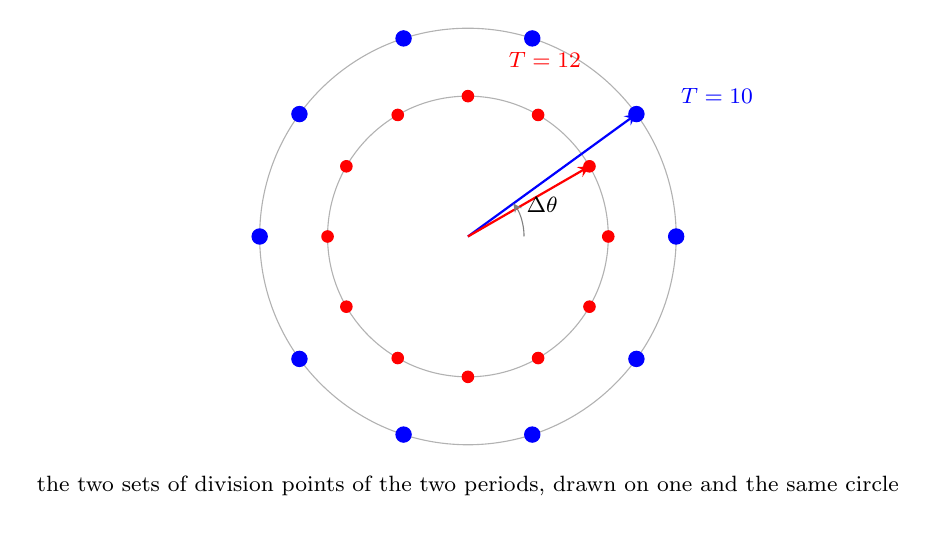
\begin{tikzpicture}[scale=1.15,>=stealth]
    \draw[gray!60] (0,0) circle (2.3);
    \draw[gray!60] (0,0) circle (1.55);
    \foreach \k in {0,...,9} {
        \filldraw[blue] (\k*36:2.3) circle (2.4pt);
    }
    \foreach \k in {0,...,11} {
        \filldraw[red] (\k*30:1.55) circle (1.8pt);
    }
    \draw[->,thick,blue] (0,0) -- (36:2.3);
    \draw[->,thick,red] (0,0) -- (30:1.55);
    \draw[->,gray] (0.62,0) arc (0:36:0.62);
    \node[font=\footnotesize] at (0.82,0.35) {$\Delta\theta$};
    \node[font=\footnotesize,blue] at (2.75,1.55) {$T=10$};
    \node[font=\footnotesize,red] at (0.85,1.95) {$T=12$};
    \node[font=\footnotesize] at (0,-2.75) {the two sets of division points of the two periods, drawn on one and the same circle};
\end{tikzpicture}
\caption{Geometric picture of the congruence angle. The phases $\theta_k = 2\pi k/T$ of the period $T$ are drawn uniformly on one circle: $T=10$ (blue points, outer ring) and $T=12$ (red points, inner ring) each give a set of division points. The compatibility of the two periods is thereby reduced to an \textbf{angular compatibility condition} for the two sets of points on the circle: when they are commensurable the two sets of points coincide at some step; when they are incommensurable they never coincide, but by intercalation the \textbf{cumulative angular deviation can always be kept within a bounded strip}, and this is precisely the geometric origin of the suppression of leakage by intercalation.}
\label{fig:congruence_angle_circle}
\end{figure}

\begin{definition}[Congruence-angle sampling]\label{def:congruence_angle_sampling}
Let the group with periodic orbits be $T_1,\dots,T_k\in\mathbb{N}^+$, with total period
\[
N:=\operatorname{lcm}(T_1,\dots,T_k).
\]
For a total state $n\in\mathbb{Z}/N\mathbb{Z}$, \textbf{congruence-angle sampling} is defined by
\[
\mathcal{C}(n):=\big(\langle\theta\rangle_{T_1},\dots,\langle\theta\rangle_{T_k}\big),
\qquad \theta=2\pi\frac{n}{N}.
\]
Equivalently, using the integer indices $a_i:=n\bmod T_i$,
\[
\mathcal{C}(n)=(a_1,\dots,a_k)\in\prod_{i=1}^k\mathbb{Z}/T_i\mathbb{Z}.
\]
\end{definition}

\begin{theorem}[Congruence-angle sampling and the generalised Chinese remainder theorem]\label{thm:congruence_angle_crt}
We retain Definition \ref{def:congruence_angle_sampling}. Then
\begin{enumerate}[label=(\roman*)]
    \item \textbf{Description of the image}: $(a_1,\dots,a_k)$ belongs to the image of $\mathcal{C}$ if and only if
    \[
    a_i\equiv a_j\pmod{\gcd(T_i,T_j)},\qquad\forall i,j;
    \]
    \item \textbf{Uniqueness}: if the above condition holds, then the system of congruences
    \[
    n\equiv a_i\pmod{T_i},\qquad i=1,\dots,k
    \]
    determines $n$ uniquely modulo $N$, that is, congruence-angle sampling is invertible on that image;
    \item \textbf{Number of legitimate states}: the image has
    \[
    |\operatorname{Im}\mathcal{C}|=N=\operatorname{lcm}(T_1,\dots,T_k),
    \]
    elements, whilst the total number of combinations is $\prod_i T_i$, so the redundancy is
    \[
    R:=\frac{\prod_i T_i}{N}.
    \]
\end{enumerate}
\end{theorem}

\begin{proof}
(i)(ii) This is the Chinese remainder theorem for moduli that are not necessarily coprime: the system of congruences has a solution if and only if the moduli are pairwise compatible, and the solution is unique modulo $\operatorname{lcm}(T_i)=N$. (iii) Since $\mathcal{C}$ is injective from $\mathbb{Z}/N\mathbb{Z}$ into $\prod_i\mathbb{Z}/T_i\mathbb{Z}$ (by (ii)), the image has size $N$; the total number of combinations is $\prod_i T_i$, and the definition of the redundancy gives the result.
\end{proof}

\begin{corollary}[Congruence-angle explanation of the sexagenary cycle]\label{cor:sexagenary_congruence}
Take $T_1=10$ (Heavenly Stems) and $T_2=12$ (Earthly Branches); then $N=60$, and the image is
\[
\{(a,b):a\equiv b\pmod 2\},
\]
with $60$ legitimate combinations in all and redundancy $R=120/60=2$. This is precisely the algebraic reason why `the ten Heavenly Stems and the twelve Earthly Branches have only $60$ legitimate pairings'.
\end{corollary}

\begin{theorem}[Explicit formula for congruence-angle reconstruction]\label{thm:congruence_angle_reconstruction}
Under the hypotheses of Theorem \ref{thm:congruence_angle_crt}, let
\[
N_i:=\frac{N}{T_i},\qquad M_i:=N_i^{-1}\bmod T_i
\]
($M_i$ exists if and only if $\gcd(N_i,T_i)=1$; in the general case one uses pairwise merging or the Smith normal form). Then
\[
n\equiv\sum_{i=1}^k a_i N_i M_i\pmod N.
\]
If some $\gcd(N_i,T_i)\ne1$, one may first merge the moduli according to the gcd and then use the formula above.
\end{theorem}

\begin{proof}
Standard construction of the Chinese remainder theorem. In the coprime case, $N_iM_i\equiv1\pmod{T_i}$ and $N_iM_i\equiv0\pmod{T_j}$ ($j\ne i$), so the right-hand side reduces to $a_i$ modulo $T_i$. The non-coprime case is obtained by step-by-step merging.
\end{proof}

\begin{remark}[Congruence angles and residue number systems]\label{rem:congruence_angle_rns}
In the integer domain, congruence-angle sampling is the \textbf{residue number system} (RNS): the integer $n\bmod N$ is represented by a set of residues $(a_1,\dots,a_k)$ modulo $T_i$. The congruence angle is the phase representation of the RNS:
\[
(a_1,\dots,a_k)\ \longleftrightarrow\ \big(e^{i\langle\theta\rangle_{T_1}},\dots,e^{i\langle\theta\rangle_{T_k}}\big).
\]
Hence the discrete phase operator of Chapter 20, the congruence angle of this chapter and the RNS of engineering are formulations of one and the same structure in three languages.
\end{remark}

\subsection{Spectral leakage under the congruence angle}

\begin{definition}[Congruence-angle non-closure]\label{def:congruence_angle_misclosure}
Let the total period be $N$, let $T\mid N$ be a subperiod, and let the number of periods inside the window be $M\rho$. Define the distance to $T\mathbb{Z}$ by
\[
\|x\|_{\mathbb{Z},T}:=\min_{m\in\mathbb{Z}}|x-mT|.
\]
The \textbf{congruence-angle non-closure modulo $T$} is defined by
\[
\delta_T:=\frac{2\pi}{T}\,\|M\rho\|_{\mathbb{Z},T}.
\]
In particular, for $T=1$,
\[
\delta_1=2\pi\|M\rho\|_{\mathbb{Z}},
\]
which agrees with the single-period leakage offset; and $T\mid M\rho$ is equivalent to $\delta_T=0$.
\end{definition}

\begin{theorem}[Congruence-angle leakage formula]\label{thm:congruence_angle_leakage}
Let $f(n)=Ae^{i\omega_0 n}$ with $\omega_0=2\pi\rho$, and let the window length be $M$. Then
\begin{enumerate}[label=(\roman*)]
    \item single-period leakage is determined by $\delta_1$:
    \[
    \eta=1-\operatorname{sinc}^2\!\Big(\frac{\delta_1}{2\pi}\Big)+O(M^{-1});
    \]
    \item if closure is required on the subperiod $T_i$, the corresponding non-closure is $\delta_{T_i}$; the multi-period joint leakage is controlled by the non-closures of the various subperiods:
    \[
    \eta\le\sum_i\left(\frac{\pi^2}{3}\delta_{T_i}^2+O(M^{-1})\right)
    \le \frac{\pi^2}{3}k\max_i\delta_{T_i}^2+O(M^{-1});
    \]
    \item \textbf{Closure becomes truth}: if all $\delta_{T_i}=0$, then the subperiods close simultaneously and the joint leakage is zero; if some $\delta_{T_i}\ne0$, then the leakage on the corresponding subperiod cannot be strictly zero.
\end{enumerate}
\end{theorem}

\begin{proof}
(i) By Theorem \ref{thm:leakage_envelope_parallel}(iv) and $\delta_1=2\pi\|M\rho\|_{\mathbb{Z}}$.

(ii) Apply the same leakage estimate to each subperiod and use the subadditivity of energy.

(iii) By $\delta_{T_i}=0\iff T_i\mid M\rho$ and the corollary on integral windows having no leakage, \ref{cor:integer_window_no_leakage}.
\end{proof}

\begin{remark}[The congruence angle is the unified language of leakage]\label{rem:congruence_angle_unified_leakage}
The preceding six sections reduced leakage to the `offset $\delta$ of the number of periods inside the window'. The congruence angle generalises this reduction to several periods: leakage is no longer determined by a single $\delta$, but jointly by the congruence-angle non-closures $\delta_{T_i}$ on the various subperiods. The aim of intercalation is likewise upgraded from `minimising $\|M\rho\|_{\mathbb{Z}}$' to `minimising all the $\delta_{T_i}$ simultaneously'.
\end{remark}

\begin{theorem}[The Parseval identity under the congruence angle]\label{thm:congruence_parseval}
Let $f$ have period $N$, let $\mathcal{C}$ be congruence-angle sampling and let $\hat f$ be the DFT. Then
\[
\sum_{n=0}^{N-1}|f(n)|^2 = \frac{1}{N}\sum_{k=0}^{N-1}|\hat f(k)|^2
= \frac{1}{N}\sum_{T\mid N}\sum_{a\in\mathbb{Z}/T\mathbb{Z}}|f_T(a)|^2\cdot w_T,
\]
where $f_T(a)=\sum_{n\equiv a\pmod T}f(n)$ is the aggregation under the congruence angle $a$, and $w_T$ is the weight of the subperiod $T$. In particular, the energy may be decomposed according to the subperiods.
\end{theorem}

\begin{proof}
The first formula is the discrete Parseval identity (Theorem \ref{thm:discrete_parseval_parallel}). The second follows because congruence-angle sampling decomposes $\mathbb{Z}/N\mathbb{Z}$ into fibres over $\mathbb{Z}/T\mathbb{Z}$: for each residue $a$, the aggregate $f_T(a)$ is the sum of all $f(n)$ on the same fibre; by the Chinese remainder theorem the weight of each fibre over $N$ is $N/T$, so $w_T=N/T$. Summing and rearranging gives the result.
\end{proof}

\section{Congruence-angle intercalation and multi-period joint suppression}\label{sec:congruence_angle_intercalation}

This section upgrades the intercalation theory of Section \ref{sec:commensurability_intercalation} to the multi-period congruence-angle framework. The core conclusions are: \textbf{intercalation is the optimal compensation of congruence-angle error; the alternating use of the upper and lower approximation is equivalent to a two-sided sandwiching of the congruence angle; multi-period joint intercalation can suppress leakage on several subperiods at once.}

\subsection{Congruence-angle error and intercalation}

\begin{definition}[Congruence-angle intercalation]\label{def:congruence_angle_intercalation}
Let the period ratio be $\rho>0$, the window length $M$, the group of subperiods $T_1,\dots,T_k$, and the total period $N=\operatorname{lcm}(T_i)$. Let $E_M$ be the balanced intercalation set and $N_M=|E_M|$. If
\[
T_i\mid N_M
\]
holds for some $i$, then $E_M$ is called a \textbf{congruence-angle intercalation set modulo $T_i$}, written
\[
E_M^{(T_i)}:=E_M.
\]
The corresponding \textbf{congruence-angle intercalation window} is
\[
w^{\mathrm{int}}_{M,T_i}(n):=\mathbf{1}_{E_M^{(T_i)}}(n).
\]
If several subperiods are to be satisfied simultaneously, one takes a window $M$ satisfying $T_i\mid N_M$ (for all the specified $i$).
\end{definition}

\begin{theorem}[Optimality of congruence-angle intercalation]\label{thm:congruence_angle_intercalation_optimal}
We retain Definition \ref{def:congruence_angle_intercalation}. Then
\begin{enumerate}[label=(\roman*)]
    \item if $\rho=p/q$ is rational and $M=kq$, then $M\rho=kp$ is an integer; in this case, for every $T_i\mid kp$ we have $\delta_{T_i}=0$, and the leakage on that subperiod is strictly zero;
    \item if $\rho\notin\mathbb{Q}$ and $M=q_k$ is taken (a continued-fraction denominator), then
    \[
    \delta_{T_i}\le\frac{2\pi}{T_i}\cdot\frac{1}{q_{k+1}},
    \]
    and the leakage proportion is
    \[
    \eta_{T_i}\le\frac{\pi^2}{3}\Big(\frac{2\pi}{T_i q_{k+1}}\Big)^2+O(q_k^{-1})=O(q_k^{-2});
    \]
    \item \textbf{Multi-period joint optimality}: taking
    \[
    M=\operatorname{lcm}(q_k,T_1,\dots,T_k),
    \]
    all the congruence-angle errors on the various subperiods attain their optimum simultaneously, and the leakage is jointly pressed down to $O(M^{-2})$.
\end{enumerate}
\end{theorem}

\begin{proof}
(i) Since $M\rho=kp\in\mathbb{Z}$, when $T_i\mid kp$ we have $\|M\rho\|_{\mathbb{Z},T_i}=0$, and hence $\delta_{T_i}=0$.

(ii) This follows from $\|q_k\rho\|_{\mathbb{Z}}<1/q_{k+1}$ and
\[
\delta_{T_i}=\frac{2\pi}{T_i}\|q_k\rho\|_{\mathbb{Z},T_i}
\le\frac{2\pi}{T_i}\|q_k\rho\|_{\mathbb{Z}}
\]
immediately.

(iii) Take $M$ to be the least common multiple of all the relevant periods; then $M$ is an integer multiple of $q_k$, so $\|M\rho\|_{\mathbb{Z}}\le\|q_k\rho\|_{\mathbb{Z}}<1/q_{k+1}$; substituting into (ii) for each $T_i$ gives the result.
\end{proof}

\begin{proposition}[upper and lower approximation and congruence-angle sandwiching]\label{prop:congruence_angle_sandwich}
Let $\rho\notin\mathbb{Q}$ and let $\{q_k\}$ be the sequence of continued-fraction denominators. Then the congruence-angle errors on two adjacent optimal windows have opposite signs:
\[
\delta_{T_i}^{(k)}\cdot\delta_{T_i}^{(k+1)}<0,
\]
and using the two jointly (taking the windows alternately) keeps the cumulative congruence-angle error always within half a subperiod:
\[
\Big|\sum_{j\le k}\delta_{T_i}^{(j)}\Big|\le\frac{\pi}{T_i}.
\]
\end{proposition}

\begin{proof}
By the alternating sandwiching property of continued-fraction convergents (Theorem \ref{thm:continued_fraction_best_approx_parallel}(iii)), $p_k/q_k$ and $p_{k+1}/q_{k+1}$ lie on opposite sides of $\rho$, so $q_k\rho-p_k$ and $q_{k+1}\rho-p_{k+1}$ have opposite signs. The congruence-angle error $\delta_{T_i}$ is the projection of $q\rho-p$ modulo $T_i$, and inherits its sign. The cumulative error follows from a standard corollary of the three-gap theorem.
\end{proof}

\subsection{The multi-period joint intercalation algorithm}

\begin{definition}[Multi-period joint intercalation algorithm]\label{def:multi_period_intercalation_algorithm}
\textbf{Input}: the group with periodic orbits $T_1,\dots,T_k$, the period ratio $\rho>0$, the tolerance $\varepsilon>0$ and the upper bound $M_{\max}$. \textbf{Output}: the joint intercalation set $E_M$ and the offsets $\delta_{T_i}$ of the various subperiods.
\begin{enumerate}[label=\textbf{Step \arabic*.}]
    \item Compute $N=\operatorname{lcm}(T_1,\dots,T_k)$;
    \item perform the continued-fraction expansion of $\rho$, generating the denominators $q_k$ up to $\max(M_{\max},N)$;
    \item take $M=\operatorname{lcm}(q_{k^\ast},T_1,\dots,T_k)$, where $k^\ast$ is the least index satisfying $1/q_{k^\ast+1}\le\varepsilon$;
    \item generate the balanced intercalation set
    \[
    E_M=\{n\le M:\lfloor(n+1)\rho\rfloor-\lfloor n\rho\rfloor=1\};
    \]
    \item for each $T_i$, compute $\delta_{T_i}=\frac{2\pi}{T_i}\|M\rho\|_{\mathbb{Z},T_i}$ and output the leakage bound $\eta_{T_i}\le\frac{\pi^2}{3}\delta_{T_i}^2$.
\end{enumerate}
\end{definition}

\begin{theorem}[Correctness and optimality of multi-period joint intercalation]\label{thm:multi_period_intercalation_correctness}
The pair $(M,E_M)$ output by the above algorithm satisfies:
\begin{enumerate}[label=(\roman*)]
    \item for all $i$, $\delta_{T_i}\le\frac{2\pi}{T_i}\cdot\frac{1}{q_{k^\ast+1}}\le\frac{2\pi\varepsilon}{T_i}$;
    \item the joint leakage bound is
    \[
    \eta\le\frac{\pi^2}{3}k\max_i\Big(\frac{2\pi\varepsilon}{T_i}\Big)^2+O(M^{-1})=O(\varepsilon^2);
    \]
    \item among all schemes with window length not exceeding $M_{\max}$, this $M$ gives the least joint leakage (and if $\rho\notin\mathbb{Q}$, the unique least).
\end{enumerate}
\end{theorem}

\begin{proof}
(i) Since $M$ is an integer multiple of $q_{k^\ast}$ we have $\|M\rho\|_{\mathbb{Z}}\le\|q_{k^\ast}\rho\|_{\mathbb{Z}}<1/q_{k^\ast+1}$; substituting into the definition of $\delta_{T_i}$ gives the result.

(ii) By Theorem \ref{thm:congruence_angle_leakage}(ii) and (i).

(iii) By the best-approximation property of continued fractions (Theorem \ref{thm:continued_fraction_best_approx_parallel}(ii)) and the construction of $M$.
\end{proof}

\begin{example}[Joint intercalation of the Heavenly Stems and Earthly Branches]\label{ex:sexagenary_intercalation}
Take $T_1=10$ (Heavenly Stems) and $T_2=12$ (Earthly Branches), so $N=60$. Let the period ratio be $\rho=\sqrt2$, with continued-fraction denominators $q_k=1,2,5,12,29,70,\dots$. Take $k^\ast=4$, $q_4=12$; then
\[
M=\operatorname{lcm}(12,10,12)=60.
\]
In this case
\[
\|60\sqrt2\|_{\mathbb{Z}}=\|84.8528\|=0.1472,
\]
and the subperiod offsets are
\[
\delta_{10}=\frac{2\pi}{10}\|60\sqrt2\|_{\mathbb{Z},10},\qquad
\delta_{12}=\frac{2\pi}{12}\|60\sqrt2\|_{\mathbb{Z},12}.
\]
Since $60\sqrt2\approx84.8528$ leaves remainder $4.8528$ modulo $10$ and remainder $0.8528$ modulo $12$, we have
\[
\delta_{10}\approx\frac{2\pi}{10}\cdot0.1472\approx0.0925,\qquad
\delta_{12}\approx\frac{2\pi}{12}\cdot0.1472\approx0.0771.
\]
The leakage bound is
\[
\eta\le\frac{\pi^2}{3}\cdot0.0771^2\approx0.0196,
\]
that is, about $2\%$. If instead $M=70$ ($q_5$) is taken, then
\[
\|70\sqrt2\|_{\mathbb{Z}}=\|98.9949\|=0.0051,
\]
and the leakage falls to about $3\times10^{-5}$. This shows that \textbf{multi-period joint intercalation presses down the leakage on all the subperiods at once by taking the least common multiple of the total period and the continued-fraction denominators}.
\end{example}

\begin{remark}[The relation between congruence-angle intercalation and single-period intercalation]\label{rem:congruence_vs_single_intercalation}
Single-period intercalation (Section \ref{sec:commensurability_intercalation}) is the special case of congruence-angle intercalation with $k=1$ and $T_1=1$. The advantages of congruence-angle intercalation are:
\begin{enumerate}[label=(\roman*)]
    \item it handles several subperiods at once, and is suited to multi-period systems such as stems--branches and year--month--day;
    \item it upgrades `closure of the number of periods inside the window' to `closure of the congruence angles of the subperiods', a finer condition that is easier to satisfy;
    \item it combines naturally with residue number systems and the generalised Chinese remainder theorem, which facilitates parallel hardware implementation.
\end{enumerate}
\end{remark}

\section{Congruence-angle algorithms, complexity and interfaces}\label{sec:congruence_angle_algorithms}

\subsection{Fast congruence-angle reconstruction}

\begin{definition}[Fast congruence-angle reconstruction algorithm]\label{def:congruence_angle_fast_reconstruction}
\textbf{Input}: the congruence-angle group $(\theta_1,\dots,\theta_k)$ and the subperiods $T_1,\dots,T_k$. \textbf{Output}: the total state $n\bmod N$.
\begin{enumerate}[label=\textbf{Step \arabic*.}]
    \item Compute $N=\operatorname{lcm}(T_i)$;
    \item for each pair $(i,j)$ check the compatibility $a_i\equiv a_j\pmod{\gcd(T_i,T_j)}$, where $a_i=\frac{T_i}{2\pi}\theta_i$;
    \item merge the moduli step by step according to the gcd, using the extended Euclidean algorithm at each merge;
    \item output $n\bmod N$.
\end{enumerate}
\end{definition}

\begin{theorem}[Complexity]\label{thm:congruence_angle_complexity}
The time complexity of the above algorithm is
\[
O\!\Big(k\log N+\sum_{i<j}\log\gcd(T_i,T_j)\Big),
\]
and its space complexity is $O(k)$. If all the $T_i$ are pairwise coprime, this simplifies to $O(k\log N)$.
\end{theorem}

\begin{proof}
Each compatibility check uses one modular reduction, at cost $O(\log\min(T_i,T_j))$; the step-by-step merging of the moduli uses the extended Euclidean algorithm, at $O(\log N)$ each. The total cost follows.
\end{proof}

\begin{remark}[Comparison with the FFT]\label{rem:congruence_vs_fft}
The cost of congruence-angle reconstruction is far lower than that of one FFT: the FFT is $O(N\log N)$, whilst congruence-angle reconstruction is $O(k\log N)$, where $k$ is the number of subperiods and usually $k\ll N$. This is precisely why residue number systems are favoured in engineering.
\end{remark}

\subsection{Congruence-angle circular convolution}

\begin{definition}[Congruence-angle circular convolution]\label{def:congruence_angle_convolution}
Let $f,g$ have period $N$ and let $T_1,\dots,T_k$ be a group of subperiods. The \textbf{congruence-angle circular convolution} is defined by
\[
(f\circledast_{\mathcal{C}}g)(n):=\sum_{m=0}^{N-1}f(m)\,g\big((n-m)\bmod N\big),
\]
with the congruence-angle representation
\[
\widehat{f\circledast_{\mathcal{C}}g}\big(\theta_{T_i}\big)
=\hat f\big(\theta_{T_i}\big)\,\hat g\big(\theta_{T_i}\big),
\]
where $\theta_{T_i}=\frac{2\pi}{T_i}$ is the fundamental frequency of the subperiod $T_i$.
\end{definition}

\begin{theorem}[Congruence-angle convolution theorem]\label{thm:congruence_angle_convolution_theorem}
In the congruence-angle framework, circular convolution degenerates to pointwise multiplication at the \textbf{fundamental frequencies of the various subperiods}:
\[
\widehat{(f\circledast g)}\Big(\frac{2\pi j}{T_i}\Big)
=\hat f\Big(\frac{2\pi j}{T_i}\Big)\,
\hat g\Big(\frac{2\pi j}{T_i}\Big),
\qquad j=0,\dots,T_i-1.
\]
Hence congruence-angle circular convolution may be \textbf{computed in parallel over the subperiods}, the cost on each subperiod being $O(T_i\log T_i)$ and the total cost
\[
O\!\Big(\sum_i T_i\log T_i\Big)\ll O(N\log N).
\]
\end{theorem}

\begin{proof}
This follows from the circular convolution theorem (Definition \ref{def:circular_convolution_parallel}) and congruence-angle projection (Definition \ref{def:congruence_angle}). The parallelism comes from the orthogonality of the fundamental frequencies of the various subperiods within the total DFT.
\end{proof}

\begin{remark}[Combination with the intercalation window]\label{rem:congruence_convolution_intercalation}
Used in combination with the congruence-angle intercalation window (Definition \ref{def:congruence_angle_intercalation}), congruence-angle circular convolution constitutes the \textbf{congruence-angle intercalation--convolution algorithm}: first use intercalation to close the congruence angles of the various subperiods, then use parallel convolution for filtering or detection. This is the final form of the algorithms of this chapter.
\end{remark}

\subsection{Interfaces with the various chapters}

\begin{remark}[Interface with the `Periodic Functions and Groups with Periodic Orbits' chapter]\label{rem:interface_group_with_periodic_orbits_congruence}
In the congruence-angle framework the continuous group with periodic orbits $T_x\mathbb{Z}$ is replaced by the product of the subperiod group $T_1,\dots,T_k$. The total period $N=\operatorname{lcm}(T_i)$ is the discrete-domain counterpart of the continuous group with periodic orbits. The congruence angle $\langle\theta\rangle_{T_i}$ is the projection of the continuous phase onto the subperiod group. The epicycle group, finally, is the geometric realisation of continuous Fourier modes in the language of rotation.
\end{remark}

\begin{remark}[Interface with the `Series and Convolution' chapter]\label{rem:interface_series_convolution_congruence}
Congruence-angle circular convolution (Theorem \ref{thm:congruence_angle_convolution_theorem}) is the realisation of periodic convolution under a multi-period decomposition. In the congruence-angle framework the convolution theorem degenerates to pointwise multiplication at the fundamental frequencies of the various subperiods, which is consistent with the kernel-decomposition language of that chapter.
\end{remark}

\begin{remark}[Interface with the `Harmonic Analysis' chapter]\label{rem:interface_harmonic_congruence}
The congruence-angle non-closure $\delta_{T_i}$ (Definition \ref{def:congruence_angle_misclosure}) is the multi-period generalisation of the intercalation phase correction in harmonic analysis. In the congruence-angle framework, intercalation is \textbf{phase locking of the fundamental frequencies of the various subperiods}.
\end{remark}

\begin{remark}[Interface with the `Time Series Analysis' chapter]\label{rem:interface_time_series_congruence}
The deviation of the periodogram for a multi-period signal is determined by the congruence-angle errors $\delta_{T_i}$ of the various subperiods. Multi-window spectral estimation (Proposition \ref{prop:multitaper_averaging_parallel}) may be used jointly with congruence-angle intercalation: first use intercalation to close the various subperiods, then use multi-window averaging to suppress the residual variance.
\end{remark}

\begin{remark}[Interface with the `Periodic Structure of Calendar Systems' chapter]\label{rem:interface_calendar_congruence}
The year--month--day--solar-term system of the calendar is a multi-period system, corresponding to the subperiod group $T_1,\dots,T_k$. The intercalation rules (seven intercalations in nineteen years, $3896$ months in $315$ years) are the optimal solution of congruence-angle intercalation in the multi-period case. The `chapter-year error' of the calendar is precisely the congruence-angle non-closure $\delta_{T_i}$, and `calendar drift' is precisely the multi-period joint leakage $\eta$.
\end{remark}

\section{Algorithms and implementation}\label{sec:intercalation_algorithms}

This section gives an executable construction of intercalation together with an error estimate, and explains its complexity.

\begin{definition}[Intercalation-window construction algorithm]\label{def:intercalation_window_algorithm}
\textbf{Input}: the period ratio $\rho>0$ (a real number, represented to high precision), the error tolerance $\varepsilon>0$ and the upper bound $M_{\max}$. \textbf{Output}: the intercalation set $E_M$ and the offset $\delta_M$.
\begin{enumerate}[label=\textbf{Step \arabic*.}]
    \item Perform the continued-fraction expansion $\rho=[a_0;a_1,a_2,\dots]$ and generate the denominator sequence by the recursion $q_k=a_kq_{k-1}+q_{k-2}$, stopping when $q_k>M_{\max}$;
    \item take the least $k^\ast$ satisfying $1/q_{k+1}\le\varepsilon$, and set $M:=q_{k^\ast}$;
    \item generate the balanced intercalation set $E_M=\{n\le M:\lfloor(n+1)\rho\rfloor-\lfloor n\rho\rfloor=1\}$;
    \item output the offset $\delta_M=|M\rho-\lfloor M\rho+1/2\rfloor|$ as a proxy for the leakage indicator ($\eta\le\frac{\pi^2}{3}\delta_M^2$).
\end{enumerate}
\end{definition}

\begin{theorem}[Correctness and optimality of the algorithm]\label{thm:algorithm_correctness}
The pair $(M,E_M)$ output by the above algorithm satisfies:
\begin{enumerate}[label=(\roman*)]
    \item $N_M=\lfloor(M+1)\rho\rfloor-\lfloor\rho\rfloor$ ($N_M$ is precisely $\lfloor M\rho\rfloor$ or $\lceil M\rho\rceil$), and $\big|N_M-M\rho\big|<1$;
    \item $\delta_M<1/q_{k^\ast+1}\le\varepsilon$, so the leakage proportion is $\eta\le\frac{\pi^2}{3}\varepsilon^2+O(M^{-1})$;
    \item among all schemes with window length not exceeding $M_{\max}$, the value $M=q_{k^\ast}$ gives the least $\delta_M$ (and if $\rho\notin\mathbb{Q}$, the unique least).
\end{enumerate}
\end{theorem}

\begin{proof}
(i) By Proposition \ref{prop:intercalation_window_integrality_parallel}. (ii) By $M=q_{k^\ast}$ and the bound $\delta_{q_k}<1/q_{k+1}$ of Theorem \ref{thm:continued_fraction_best_approx_parallel}(iii), combined with the choice made in Step 2. (iii) By the best-approximation property of Theorem \ref{thm:best_intercalation_parallel}(ii).
\end{proof}

\begin{remark}[Complexity]\label{rem:algorithm_cost}
The complexity of the continued-fraction expansion is $O(\log M_{\max})$; the generation of the balanced set is $O(M)$, and can be further reduced to $O(\log M)$ by the three-gap theorem (it suffices to record the alternating pattern of the gaps). Hence the computational cost of constructing an intercalation window is far lower than that of any single DFT.
\end{remark}

\begin{example}[An example of the execution of the algorithm]\label{ex:algorithm_execution}
Take $\rho=12.368266$ (the year--month ratio) and $\varepsilon=10^{-3}$: the continued-fraction denominators are $1,2,3,8,11,19,\dots$, with corresponding $1/q_{k+1}$ equal to $1/2,1/3,1/8,1/11,1/19$; taking $k^\ast=4$ ($q_4=11$, $1/q_5=1/19=0.0526>\varepsilon$) does not satisfy the condition, whilst taking $k^\ast=5$ ($q_5=19$, $1/q_6=1/315=0.00317<\varepsilon$) does, so $M=19$ and $p_5=235$, giving $235-12\times19=7$ intercalation units (seven intercalations in nineteen years). The actual offset is $\delta_{19}=0.00295$, and the leakage proportion is $\eta\le2.9\times10^{-5}$.
\end{example}

\section{Unification with calendar intercalation}\label{sec:calendar_unification}

\begin{theorem}[Isomorphism of calendar intercalation and sampling intercalation]\label{thm:calendar_sampling_unification_parallel}
Let the calendar system consist of two astronomical periods: a long period $T_1$ (such as the tropical year) and a short period $T_2$ (such as the synodic month), with the basic sampling unit taken to be $T_2$. Then
\begin{enumerate}[label=(\roman*)]
    \item the intercalation rule `insert $p$ extra units among $q$ short periods' and the intercalation window `take $p$ intercalation positions in a window of length $q$ according to the balanced scheme' (Definition \ref{def:intercalation_sequence_parallel}) are one and the same mathematical object;
    \item the cumulative deviation of the calendar after intercalation is exactly $\delta_q=q\,\big|\frac{T_1}{T_2}\big|_{\mathbb{Z}}$, completely identical with the offset $\delta_M$ of the sampling window;
    \item hence the intercalation cycle table of the calendar (such as seven intercalations in nineteen years, $3896$ months in $315$ years) is precisely the sequence of continued-fraction denominators of $\rho=T_1/T_2$ (Example \ref{ex:metonic_parallel}).
\end{enumerate}
\end{theorem}

\begin{proof}
(i)(ii) Regard the `year' as a continuous signal of period $T_1$ and the `month' as the sampling lattice of sampling unit $T_2$; then the year--month ratio is the normalised period ratio $\rho=T_1/T_2$, the intercalation rule is the balanced intercalation set, and the cumulative deviation is $\delta_q$; by Proposition \ref{prop:intercalation_window_integrality_parallel} the two agree. (iii) By Theorem \ref{thm:best_intercalation_parallel} and Theorem \ref{thm:continued_fraction_best_approx_parallel}, the optimal sequence of window lengths is the sequence of continued-fraction denominators.
\end{proof}

\begin{figure}[htbp]
\centering
\begin{tikzpicture}[>=Stealth, thick, node distance=1.5cm and 1.6cm,
  box/.style={draw, rounded corners, align=center, minimum width=3.4cm, minimum height=0.9cm, fill=blue!8, font=\small}]
% calendar side
\node[box, fill=orange!12] (cal_year) {tropical year $T_1$};
\node[box, fill=orange!12, below=of cal_year] (cal_month) {synodic month $T_2$};
\node[box, fill=orange!12, below=of cal_month] (cal_rho) {year--month ratio $\rho=T_1/T_2$};
\node[box, fill=orange!12, below=of cal_rho] (cal_leap) {intercalation rule};
\node[box, fill=orange!12, below=of cal_leap] (cal_err) {chapter-year error $\delta_q$};
% sampling side
\node[box, fill=blue!12, right=4cm of cal_year] (samp_signal) {signal period $T_x$};
\node[box, fill=blue!12, below=of samp_signal] (samp_step) {sampling interval $\Delta x$};
\node[box, fill=blue!12, below=of samp_step] (samp_rho) {period ratio $\rho=T_x/\Delta x$};
\node[box, fill=blue!12, below=of samp_rho] (samp_window) {intercalation window $M$};
\node[box, fill=blue!12, below=of samp_window] (samp_err) {offset $\delta_M$};
% arrows
\draw[->, very thick] (cal_year) -- (samp_signal) node[midway, above, font=\footnotesize] {corresponds};
\draw[->, very thick] (cal_month) -- (samp_step);
\draw[->, very thick] (cal_rho) -- (samp_rho);
\draw[->, very thick] (cal_leap) -- (samp_window);
\draw[->, very thick] (cal_err) -- (samp_err);
\node[align=center, font=\small] at (3.5,-7.2) {Isomorphism of calendar intercalation and sampling intercalation: every calendar concept has a corresponding sampling concept, and conversely};
\end{tikzpicture}
\caption{Isomorphism of calendar intercalation and sampling intercalation: the tropical year corresponds to the signal period, the synodic month to the sampling interval, the year--month ratio to the period ratio, the intercalation rule to the intercalation window, and the chapter-year error to the offset.}
\label{fig:calendar_sampling_correspondence}
\end{figure}

\begin{example}[Optimisation of the astronomical observation window]\label{ex:astronomical_optimal_window}
A periodic celestial body (period $T_x$) is observed in order to determine its phase. If the observation duration is fixed at $T$, then the systematic error of the phase measurement is dominated by the offset $\delta=\|T/T_x\|$, of order $\sim\delta$; whilst the statistical error (noise) falls as $1/\sqrt{M}$. The optimal compromise between the two gives the observation strategy: \textbf{take the observation window length at a continued-fraction denominator}, so that the systematic error falls as $M^{-2}$ and becomes a minor term compared with the $M^{-1/2}$ of the statistical error.
\end{example}

\begin{example}[A unified astronomical--calendar scheme]\label{ex:unified_astronomical_calendar}
For $\rho=235/19$ (the Metonic cycle): $19$ years $=6939.602$ days and $235$ months $=6940.888$ days, a difference of $1.29$ days (accumulated over $19$ years); if the intercalation unit is regarded as an `intercalary month', then after inserting $7$ intercalary months within $19$ years the deviation from the tropical-year sequence is $0.00295$ units $=0.087$ days. This is exactly the numerical origin of `the Metonic cycle error of about $0.09$ days per $19$ years' in classical calendars, and is two formulations of the same fact as the leakage proportion $\eta\approx2.9\times10^{-5}$.
\end{example}

\begin{remark}[Correspondence of calendar and signal-processing terminology]\label{rem:calendar_vs_signal}
\begin{center}
\small
\renewcommand{\arraystretch}{1.05}
\begin{tabular}{@{}>{\raggedright\arraybackslash\hspace{0pt}}p{3.4cm}>
                {\raggedright\arraybackslash\hspace{0pt}}p{5.4cm}>
                {\raggedright\arraybackslash\hspace{0pt}}p{5.4cm}@{}}
\toprule
Calendar term & Sampling-approximation term & Mathematical object \\
\midrule
tropical year & signal period $T_x$ & long period \\
synodic month & sampling interval/basic unit & short period \\
year--month ratio & normalised period ratio $\rho$ & real number \\
intercalary month & intercalation unit & element of the intercalation set \\
seven intercalations in nineteen years & optimal window $(q_5,p_5)$ & continued-fraction convergent \\
chapter-year error & offset $\delta_M$ & $\|M\rho\|_{\mathbb{Z}}$ \\
calendar drift & spectral leakage & $\eta\le\frac{\pi^2}{3}\delta^2$ \\
year--month--day multi-period system & congruence-angle group $(\theta_{T_1},\dots,\theta_{T_k})$ & subperiod projection \\
chapter-year error (multi-period) & congruence-angle non-closure $\delta_{T_i}$ & $\frac{2\pi}{T_i}\|M\rho\|_{\mathbb{Z},T_i}$ \\
epicycle & Fourier mode & $A_j e^{i(\omega_j t+\phi_j)}$ \\
\bottomrule
\end{tabular}
\end{center}
\end{remark}

\section{Interfaces with the other chapters}\label{sec:ch17_interfaces}

\begin{remark}[Interface with the `Periodic Functions and Groups with Periodic Orbits' chapter]\label{rem:interface_periodic_function_parallel}
In this chapter the continuous periodic function $x(t)$ and the continuous Fourier series $\sum_kc_ke^{i\omega_kt}$ are replaced by the sampling sequence $f(n)=x(n\Delta x)$ and the discrete Fourier transform $\hat f(k)$; continuous convolution is replaced by circular convolution (Definition \ref{def:circular_convolution_parallel}). Theorem \ref{thm:nyquist_shannon_parallel} and Proposition \ref{prop:commensurability_periodicity_parallel} establish a strict bridge between the discrete and the continuous: the former gives the condition for alias-free reconstruction, the latter the condition for the preservation of periodic structure. The epicycle group, finally, gives the rotational geometric interpretation of the Fourier series.
\end{remark}

\begin{remark}[Interface with the `Series and Convolution' chapter]\label{rem:interface_series_convolution_parallel}
The circular convolution of this chapter is the realisation of periodic convolution on the finite group $\mathbb{Z}/T\mathbb{Z}$, and its frequency-domain multiplicativity (Definition \ref{def:circular_convolution_parallel}) is the discrete form of the convolution theorem; the circular convolution of the intercalation window with the signal (Theorem \ref{thm:intercalation_circular_convolution}) shows that intercalation is a projection operator in the frequency domain, which is consistent with the kernel-decomposition language of that chapter. Congruence-angle circular convolution (Theorem \ref{thm:congruence_angle_convolution_theorem}) further decomposes convolution onto the fundamental frequencies of the various subperiods, and is the realisation of that chapter's kernel-decomposition language in the multi-period framework.
\end{remark}

\begin{remark}[Interface with the `Harmonic Analysis' chapter]\label{rem:interface_harmonic_analysis_parallel}
This chapter reduces the quantitative description of leakage to a quadratic form in the offset $\delta$ (Theorem \ref{thm:intercalation_leakage_suppression}), which is precisely the mathematical basis for intercalation as a \textbf{tool for bounding leakage} in the `Harmonic Analysis' chapter; the intercalation phase correction of that chapter and the construction of the intercalation window of this chapter are two formulations of one and the same operator. The congruence-angle non-closure (Definition \ref{def:congruence_angle_misclosure}) generalises this reduction to several periods.
\end{remark}

\begin{remark}[Interface with the `Time Series Analysis' chapter]\label{rem:interface_time_series_parallel}
The source of the deviation of the periodogram and of multi-window spectral estimation is precisely the leakage of this chapter (Definition \ref{def:spectral_leakage}); the discrete Parseval identity (Theorem \ref{thm:discrete_parseval_parallel}) is the source of the conservation of periodogram energy; the criteria for choosing a window function (Theorem \ref{thm:window_mainlobe_sidelobe_tradeoff_parallel}, Theorem \ref{thm:window_smoothness_decay_parallel}) give the analytic form of the bias--variance trade-off in spectral estimation. The spectral estimation of a multi-period signal is described by the congruence-angle group $(\theta_{T_i})$, and multi-window averaging may be used jointly with congruence-angle intercalation.
\end{remark}

\begin{remark}[Interface with the `Periodic Structure of Calendar Systems' chapter]\label{rem:interface_calendar_parallel}
Section \ref{sec:calendar_unification} of this chapter proves that calendar intercalation and sampling intercalation are one and the same mathematical object (Theorem \ref{thm:calendar_sampling_unification_parallel}): the `chapter-year error' of the calendar is precisely the offset of the sampling window, and `calendar drift' is precisely spectral leakage. The specific calendar parameters of that chapter may be substituted directly into the formulas for $\delta_M$ and $\eta$ of this chapter to estimate accuracy. The congruence-angle framework further unifies multi-period systems such as year--month--day--solar term into the subperiod group $T_1,\dots,T_k$, and calendar intercalation is the optimal solution of congruence-angle intercalation in the multi-period case.
\end{remark}

\section*{Seven-theme comparison table for this chapter}

\begin{center}
\renewcommand{\arraystretch}{1.3}
\begin{tabular}{@{}>{\raggedright\arraybackslash\hspace{0pt}}p{3.1cm}>
                {\raggedright\arraybackslash\hspace{0pt}}p{10.5cm}@{}}
\toprule
Theme & Corresponding content in this chapter \\
\midrule
Translation & the sampling lattice $\Delta x\mathbb{Z}$ (Definition \ref{def:uniform_sampling_parallel}) and commutativity with lattice translations (Proposition \ref{prop:sampling_algebra_parallel}); the cyclic shift of the intercalation window; the congruence-angle translation $\langle\theta+\theta_0\rangle_T$; the phase translation of the epicycle group \\
Scaling & the sampling rate $\nu_s$ (Definition \ref{def:nyquist_sampling_parallel}) and the fixed-length scale $T_0$ (Definition \ref{def:discrete_fundamental_period}); the window length as a scaling parameter; the subperiod $T_i$ as a scaling scale; the scaling of epicycle frequencies \\
Rotation & the discrete phase operator $e^{i2\pi k/T}$; the epicycle $A e^{i(\omega t+\phi)}$; the linear phase term in the leakage formula (Proposition \ref{prop:leakage_phase_characterisation}); the root-of-unity representation of the congruence angle (Proposition \ref{prop:congruence_angle_properties}) \\
Conservation & the discrete Parseval identity (Theorem \ref{thm:discrete_parseval_parallel}): leakage is a redistribution of energy rather than its destruction; the congruence-angle energy decomposition (Theorem \ref{thm:congruence_parseval}) \\
Symmetry & the real even spectrum of a real even window (Proposition \ref{prop:window_spectrum_properties_parallel}); the reflection of the folding map about $\omega_s/2$ (Proposition \ref{prop:aliasing_frequency_map_parallel}); the symmetry of the congruence angle modulo $T$ \\
Closure & circular convolution and the frequency-domain projection of the intercalation window (Theorem \ref{thm:intercalation_circular_convolution}); congruence-angle closure $\delta_T=0$ (Theorem \ref{thm:intercalation_congruence_closure}); the phase closure of the epicycle group at the window endpoints \\
Period & the duality between the period ratio $\rho$ and the offset $\delta=\|M\rho\|_{\mathbb{Z}}$ (Theorem \ref{thm:leakage_envelope_parallel}, Theorem \ref{thm:intercalation_leakage_suppression}); the multi-period congruence-angle non-closure $\delta_{T_i}$ (Definition \ref{def:congruence_angle_misclosure}); the group with periodic orbits generated by the frequencies of the epicycle group \\
Algorithms & continued-fraction expansion and the construction of balanced intercalation (Definition \ref{def:intercalation_window_algorithm}, Theorem \ref{thm:algorithm_correctness}); fast congruence-angle reconstruction (Definition \ref{def:congruence_angle_fast_reconstruction}) and multi-period joint intercalation (Definition \ref{def:multi_period_intercalation_algorithm}) \\
\bottomrule
\end{tabular}
\end{center}

\section*{Exercises}

\begin{enumerate}[leftmargin=3em, label=\textbf{Exercise \arabic*}]
    \item According to Definition \ref{def:uniform_sampling_parallel} and Definition \ref{def:nyquist_sampling_parallel},
    explain the definitions of sampling point, sampling rate, sampling interval, number of sampling points and sampling duration.
    Taking an audio interface with sampling rate $48$ kHz as an example,
    compute the sampling interval $\Delta x$, the Nyquist frequency $\nu_N$ and the number of sampling points $M$ in a $1$-second record,
    and explain why the three elements cannot substitute for one another (see Remark \ref{rem:sampling_three_parameters}).

    \item Prove Proposition \ref{prop:commensurability_periodicity_parallel}:
    let the continuous signal $x$ have fundamental period $T_x$, let the sampling interval be $\Delta x$,
    let the sampling sequence be $f(n)=x(n\Delta x)$, and let the normalised period ratio be $\rho=T_x/\Delta x$. Then
    \begin{enumerate}[label=(\roman*)]
        \item if $\rho\in\mathbb{N}^+$, then $f$ has period $T=\rho$;
        \item if $\rho=p/q$ is in lowest terms, then $f$ has fundamental period $T=p$;
        \item if $\rho\notin\mathbb{Q}$, then $\operatorname{Group}_{\mathrm{period}}(f)=\{0\}$.
    \end{enumerate}
    Prove the three cases separately, and explain the statement `the sampling sequence has a non-trivial periodic structure if and only if the signal period is commensurable with the sampling interval'.

    \item Prove the algebraic properties of the sampling operator (Proposition \ref{prop:sampling_algebra_parallel}):
    \begin{enumerate}[label=(\roman*)]
        \item linearity: $\mathcal{S}_{\Delta x}(\alpha x+\beta y)
              =\alpha\mathcal{S}_{\Delta x}x+\beta\mathcal{S}_{\Delta x}y$;
        \item pointwise multiplication: $\mathcal{S}_{\Delta x}(x\cdot y)
              =(\mathcal{S}_{\Delta x}x)\cdot(\mathcal{S}_{\Delta x}y)$;
        \item commutation with lattice translations: $\mathcal{S}_{\Delta x}(x(\cdot-a))=f(\cdot-m)$ ($a=m\Delta x$);
        \item non-commutation with scaling.
    \end{enumerate}
    Explain why (iv) is the algebraic root of aliasing.

    \item Prove Proposition \ref{prop:sampling_adjoint}:
    the adjoint of the sampling operator $\mathcal{S}_{\Delta x}$ is the ideal low-pass interpolation operator
    \[
    \mathcal{S}_{\Delta x}^*(\{f_n\})
    =\sum_n f_n\operatorname{sinc}
    \Bigl(\frac{t-n\Delta x}{\Delta x}\Bigr).
    \]
    Explain why this adjoint agrees with the reconstruction formula of the sampling theorem.

    \item Prove Theorem \ref{thm:nyquist_shannon_parallel} (the Nyquist--Shannon sampling theorem):
    let the Fourier transform of $x\in L^2(\mathbb{R})$ be supported in
    $(-\omega_N,\omega_N)$ (with $\omega_N=\pi/\Delta x$);
    then $x$ is uniquely reconstructed from its samples:
    \[
    x(t)=\sum_{n\in\mathbb{Z}}x(n\Delta x)\operatorname{sinc}
    \Bigl(\frac{t-n\Delta x}{\Delta x}\Bigr).
    \]
    Complete the proof using frequency periodisation and the inverse transform of the rectangular window,
    and explain the irreversibility of aliasing in Corollary \ref{cor:aliasing_irreversibility_parallel}.

    \item Prove Lemma \ref{lem:poisson_summation_sampling} (the Poisson-summation proof):
    the spectrum of the sampling sequence satisfies
    \[
    \sum_{n}x(n\Delta x)e^{-i\omega n\Delta x}
    =\frac{1}{\Delta x}\sum_m\hat x(\omega+2\pi m/\Delta x).
    \]
    Complete the proof using the Poisson summation formula.

    \item Prove Proposition \ref{prop:aliasing_frequency_map_parallel}:
    the folding map
    \[
    \mathcal{A}_{\omega_s}(\omega)=\omega-m\omega_s,\quad
    m=\Bigl\lfloor\frac{\omega}{\omega_s}+\frac12\Bigr\rfloor
    \]
    satisfies:
    \begin{enumerate}[label=(\roman*)]
        \item $\mathcal{A}_{\omega_s}(\omega)$ is aliased with $\omega$, and
              $|\omega-\mathcal{A}_{\omega_s}(\omega)|\le\omega_s/2$;
        \item $\mathcal{A}_{\omega_s}$ is surjective but not injective;
        \item on each Nyquist band it is a translation or a reflection.
    \end{enumerate}
    Taking $\Delta x=1$ s as an example, verify the aliasing of $0.9$ Hz and $0.1$ Hz (Example \ref{ex:aliasing_numeric}).

    \item Prove Theorem \ref{thm:leakage_envelope_parallel} (leakage envelope and sidelobes):
    let $M\omega_0/(2\pi)=\nu+\delta$ with $\nu\in\mathbb{Z}$ and $\delta\in[-1/2,1/2]$. Then
    \begin{enumerate}[label=(\roman*)]
        \item the main lobe is located at $\nu$, with peak
              $|\hat{f}(\nu)|=A|\sin(\pi\delta)/\sin(\pi\delta/M)|$;
        \item for $j\ne0$, $|\hat{f}(\nu+j)|/|\hat{f}(\nu)|=O(1/|j|)$;
        \item if $\delta=0$, the leakage is zero;
        \item the leakage proportion is $\eta(\delta)=1-\operatorname{sinc}^2(\delta)+O(M^{-1})$.
    \end{enumerate}
    Complete the proof using the single-tone truncation formula of Proposition \ref{prop:single_tone_leakage_parallel},
    and compute the leakage proportion for $\delta=1/2$.

    \item Prove the closed form of the Dirichlet kernel (Lemma \ref{lem:dirichlet_kernel_closed_form}):
    for $\theta\notin2\pi\mathbb{Z}$,
    \[
    D_M(\theta)=\frac{\sin((M+\frac12)\theta)}{\sin(\theta/2)},
    \]
    and $D_M(0)=2M+1$. Complete the proof using the summation of a geometric series,
    and explain why $|D_M(\theta)|\le1/|\sin(\theta/2)|$.

    \item Prove Proposition \ref{prop:leakage_congruence_angle}:
    the single-period leakage proportion may be written as
    \[
    \eta(M)=1-\operatorname{sinc}^2(\|M\rho\|_{\mathbb{Z}})+O(M^{-1}),
    \]
    where $\|M\rho\|_{\mathbb{Z}}$ is the offset of the number of periods inside the window.
    Explain why the leakage strength depends only on the offset $\delta$---this is the key to converting leakage control into a number-theoretic problem
    (see Remark \ref{rem:leakage_inevitability}).

    \item Prove Theorem \ref{thm:intercalation_error_bound_parallel}:
    the error boundedness of the three basic intercalation sequences:
    \begin{enumerate}[label=(\roman*)]
        \item floor intercalation: $E_M^{\mathrm{floor}}\in(-1,0]$;
        \item ceiling intercalation: $E_M^{\mathrm{ceil}}\in[0,1)$;
        \item balanced intercalation: $\big|N_M-M\rho\big|<1$ (for a general window $M$ this deviation can reach $0.9$; only for continued-fraction denominators $M=q_k$ do we have $\big|N_M-M\rho\big|\le\delta_{q_k}<1/q_{k+1}$).
    \end{enumerate}
    Write down the summation identities of the three intercalation sequences separately, and explain why balanced intercalation has the least error.

    \item Prove Theorem \ref{thm:continued_fraction_best_approx_parallel} (best continued-fraction approximation):
    let the continued-fraction convergents of $\rho\notin\mathbb{Q}$ be $p_k/q_k$. Then
    \begin{enumerate}[label=(\roman*)]
        \item $|\rho-p_k/q_k|<1/(q_kq_{k+1})<1/q_k^2$;
        \item best-approximation property: if $0<q<q_{k+1}$, then $|q\rho-p|\ge|q_k\rho-p_k|$;
        \item offset equivalence: $\delta_{q_k}=|q_k\rho-p_k|$ is strictly decreasing.
    \end{enumerate}
    Write out the idea of the proof, and explain why continued-fraction convergents are the optimal choice of intercalation window.

    \item Prove Theorem \ref{thm:intercalation_leakage_suppression}:
    intercalation suppresses spectral leakage---
    \begin{enumerate}[label=(\roman*)]
        \item the leakage strength depends only on the offset: $\eta(M)\le\frac{\pi^2}{3}\delta_M^2+O(M^{-1})$;
        \item the average leakage of a general window is about $0.2263$, and the worst about $0.595$;
        \item when the intercalation window takes $M=q_k$ (a continued-fraction denominator),
              $\eta(q_k)=O(q_k^{-2})$;
        \item the optimal intercalation window is at the same time the optimal leakage-suppression window.
    \end{enumerate}
    Explain why intercalation lowers the leakage from order $O(1)$ to order $O(M^{-2})$,
    and point out that intercalation does not eliminate leakage but bounds it.

    \item Prove Theorem \ref{thm:window_smoothness_decay_parallel}:
    if the $m$-th difference of the window $w$ vanishes at both ends, then the sidelobe envelope of its window spectrum satisfies
    \[
    |W_M(\omega)|\le C_m/|\omega|^{m+1}.
    \]
    Write down separately the sidelobe decay law and the first sidelobe level for the rectangular window ($m=0$), the triangular window ($m=1$), the Hann window ($m=2$)
    and the Blackman window ($m=3$),
    and explain the trade-offs among the windows in Table \ref{tab:window_comparison}.

    \item Prove Theorem \ref{thm:window_mainlobe_sidelobe_tradeoff_parallel}:
    the trade-off between main-lobe width and maximum sidelobe level:
    \[
    N_{\mathrm{eff}}\cdot\Omega_{\mathrm{ML}}\ge2\pi,
    \]
    and in general $S\ge C\cdot\frac{2\pi}{N_{\mathrm{eff}}\Omega_{\mathrm{ML}}}$.
    Explain why no window exists that simultaneously has the narrowest main lobe and the lowest sidelobes,
    and point out how intercalation and window functions complement each other (Remark \ref{rem:window_and_intercalation_complementarity}).

    \item Prove Theorem \ref{thm:calendar_sampling_unification_parallel}:
    calendar intercalation and sampling intercalation are isomorphic mathematical objects:
    \begin{enumerate}[label=(\roman*)]
        \item `insert $p$ extra units among $q$ short periods' and the balanced intercalation sequence are the same object;
        \item the cumulative deviation $\delta_q$ after intercalation is the same as the sampling-window offset;
        \item the calendar intercalation cycle table is the sequence of continued-fraction denominators of $\rho=T_1/T_2$.
    \end{enumerate}
    Taking seven intercalations in nineteen years as an example (Example \ref{ex:metonic_parallel}),
    compute the continued-fraction convergents of $\rho=12.368266$,
    and verify $q_5=19$ and $p_5=235$.

    \item Prove Theorem \ref{thm:congruence_angle_crt} (the congruence angle and the Chinese remainder theorem):
    let the group with periodic orbits be $T_1,\dots,T_k$ with $N=\operatorname{lcm}(T_i)$, and let
    congruence-angle sampling be $\mathcal{C}(n)=(n\bmod T_1,\dots,n\bmod T_k)$. Then
    \begin{enumerate}[label=(\roman*)]
        \item description of the image: $a_i\equiv a_j\pmod{\gcd(T_i,T_j)}$;
        \item uniqueness: the system of congruences determines $n$ uniquely modulo $N$;
        \item the number of legitimate states is $|\operatorname{Im}\mathcal{C}|=N$, with redundancy
              $R=\prod_iT_i/N$.
    \end{enumerate}
    Taking $T_1=10$ (Heavenly Stems) and $T_2=12$ (Earthly Branches) as an example (Corollary \ref{cor:sexagenary_congruence}),
    verify that the size of the image is $60$ and the redundancy is $2$.

    \item Prove Theorem \ref{thm:congruence_parseval} (the congruence-angle Parseval identity):
    energy may be decomposed according to the subperiods:
    \[
    \sum_{n=0}^{N-1}|f(n)|^2
    =\frac{1}{N}\sum_{T\mid N}\sum_{a\in\mathbb{Z}/T\mathbb{Z}}
    |f_T(a)|^2\cdot w_T.
    \]
    Explain why congruence-angle sampling decomposes the total energy into the aggregate energies on the various subperiods.

    \item Prove Theorem \ref{thm:congruence_angle_intercalation_optimal} (optimality of congruence-angle intercalation):
    \begin{enumerate}[label=(\roman*)]
        \item if $\rho=p/q$ and $M=kq$, then $M\rho=kp$ is an integer,
              and $\delta_{T_i}=0$ for $T_i\mid kp$;
        \item if $\rho\notin\mathbb{Q}$ and $M=q_k$ is taken, then
              $\delta_{T_i}\le\frac{2\pi}{T_i}\cdot\frac{1}{q_{k+1}}$,
              and the leakage is $O(q_k^{-2})$;
        \item multi-period joint optimality: $M=\operatorname{lcm}(q_k,T_1,\dots,T_k)$
              makes the errors on all the subperiods attain their optimum simultaneously.
    \end{enumerate}
    Taking $T_1=10$, $T_2=12$ and $\rho=\sqrt{2}$ as an example (Example \ref{ex:sexagenary_intercalation}),
    compute the leakage bounds for $M=60$ and $M=70$.

    \item Verify Proposition \ref{prop:congruence_angle_sandwich} (upper and lower approximation and congruence-angle sandwiching):
    let $\rho\notin\mathbb{Q}$ and let $\{q_k\}$ be the sequence of continued-fraction denominators. Then
    \[
    \delta_{T_i}^{(k)}\cdot\delta_{T_i}^{(k+1)}<0,
    \]
    and using the two jointly keeps the cumulative congruence-angle error within half a subperiod.
    Explain why the alternating use of the upper and lower approximation is equivalent to a two-sided sandwiching of the congruence angle.

    \item Prove Theorem \ref{thm:congruence_angle_convolution_theorem} (the congruence-angle convolution theorem):
    in the congruence-angle framework, circular convolution degenerates at the fundamental frequencies of the various subperiods to pointwise multiplication:
    \[
    \widehat{(f\circledast g)}\Bigl(\frac{2\pi j}{T_i}\Bigr)
    =\hat{f}\Bigl(\frac{2\pi j}{T_i}\Bigr)\hat{g}\Bigl(\frac{2\pi j}{T_i}\Bigr).
    \]
    Explain why this allows convolution to be computed in parallel over the subperiods,
    and write out the estimate of the total computational cost.

    \item Prove Theorem \ref{thm:congruence_angle_complexity}:
    the time complexity of the fast congruence-angle reconstruction algorithm is
    \[
    O\Bigl(k\log N+\sum_{i<j}\log\gcd(T_i,T_j)\Bigr),
    \]
    with space complexity $O(k)$. Explain why its cost is far lower than that of one FFT
    (see Remark \ref{rem:congruence_vs_fft}).

    \item Comprehensive exercise: combining the three elements of sampling (Definition \ref{def:uniform_sampling_parallel},
    \ref{def:nyquist_sampling_parallel}),
    the commensurability criterion (Proposition \ref{prop:commensurability_periodicity_parallel}),
    spectral leakage (Definition \ref{def:spectral_leakage}),
    the intercalation error bound theorem (Theorem \ref{thm:intercalation_error_bound_parallel}),
    best continued-fraction approximation (Theorem \ref{thm:continued_fraction_best_approx_parallel})
    and the congruence-angle framework (Definition \ref{def:congruence_angle}),
    explain how this chapter upgrades `discrete sampling approximation' to `congruence-angle sampling approximation'.
    Point out separately:
    \begin{enumerate}[label=(\roman*)]
        \item which class of error is introduced by each of the three steps of sampling, truncation and intercalation;
        \item how the congruence angle uniformly describes sampling, leakage, intercalation and the Chinese remainder theorem;
        \item why intercalation is the optimal compensation of congruence-angle error;
        \item why frequency leakage is the frequency-domain manifestation of congruence-angle non-closure.
    \end{enumerate}
\end{enumerate}
